% Options for packages loaded elsewhere
% Options for packages loaded elsewhere
\PassOptionsToPackage{unicode}{hyperref}
\PassOptionsToPackage{hyphens}{url}
\PassOptionsToPackage{dvipsnames,svgnames,x11names}{xcolor}
%
\documentclass[
  letterpaper,
  DIV=11,
  numbers=noendperiod]{scrartcl}
\usepackage{xcolor}
\usepackage[margin=1in]{geometry}
\usepackage{amsmath,amssymb}
\setcounter{secnumdepth}{5}
\usepackage{iftex}
\ifPDFTeX
  \usepackage[T1]{fontenc}
  \usepackage[utf8]{inputenc}
  \usepackage{textcomp} % provide euro and other symbols
\else % if luatex or xetex
  \usepackage{unicode-math} % this also loads fontspec
  \defaultfontfeatures{Scale=MatchLowercase}
  \defaultfontfeatures[\rmfamily]{Ligatures=TeX,Scale=1}
\fi
\usepackage{lmodern}
\ifPDFTeX\else
  % xetex/luatex font selection
  \setmainfont[]{Latin Modern Roman}
  \setsansfont[]{Latin Modern Sans}
  \setmonofont[]{Latin Modern Mono}
\fi
% Use upquote if available, for straight quotes in verbatim environments
\IfFileExists{upquote.sty}{\usepackage{upquote}}{}
\IfFileExists{microtype.sty}{% use microtype if available
  \usepackage[]{microtype}
  \UseMicrotypeSet[protrusion]{basicmath} % disable protrusion for tt fonts
}{}
\makeatletter
\@ifundefined{KOMAClassName}{% if non-KOMA class
  \IfFileExists{parskip.sty}{%
    \usepackage{parskip}
  }{% else
    \setlength{\parindent}{0pt}
    \setlength{\parskip}{6pt plus 2pt minus 1pt}}
}{% if KOMA class
  \KOMAoptions{parskip=half}}
\makeatother
% Make \paragraph and \subparagraph free-standing
\makeatletter
\ifx\paragraph\undefined\else
  \let\oldparagraph\paragraph
  \renewcommand{\paragraph}{
    \@ifstar
      \xxxParagraphStar
      \xxxParagraphNoStar
  }
  \newcommand{\xxxParagraphStar}[1]{\oldparagraph*{#1}\mbox{}}
  \newcommand{\xxxParagraphNoStar}[1]{\oldparagraph{#1}\mbox{}}
\fi
\ifx\subparagraph\undefined\else
  \let\oldsubparagraph\subparagraph
  \renewcommand{\subparagraph}{
    \@ifstar
      \xxxSubParagraphStar
      \xxxSubParagraphNoStar
  }
  \newcommand{\xxxSubParagraphStar}[1]{\oldsubparagraph*{#1}\mbox{}}
  \newcommand{\xxxSubParagraphNoStar}[1]{\oldsubparagraph{#1}\mbox{}}
\fi
\makeatother

\usepackage{color}
\usepackage{fancyvrb}
\newcommand{\VerbBar}{|}
\newcommand{\VERB}{\Verb[commandchars=\\\{\}]}
\DefineVerbatimEnvironment{Highlighting}{Verbatim}{commandchars=\\\{\}}
% Add ',fontsize=\small' for more characters per line
\usepackage{framed}
\definecolor{shadecolor}{RGB}{241,243,245}
\newenvironment{Shaded}{\begin{snugshade}}{\end{snugshade}}
\newcommand{\AlertTok}[1]{\textcolor[rgb]{0.68,0.00,0.00}{#1}}
\newcommand{\AnnotationTok}[1]{\textcolor[rgb]{0.37,0.37,0.37}{#1}}
\newcommand{\AttributeTok}[1]{\textcolor[rgb]{0.40,0.45,0.13}{#1}}
\newcommand{\BaseNTok}[1]{\textcolor[rgb]{0.68,0.00,0.00}{#1}}
\newcommand{\BuiltInTok}[1]{\textcolor[rgb]{0.00,0.23,0.31}{#1}}
\newcommand{\CharTok}[1]{\textcolor[rgb]{0.13,0.47,0.30}{#1}}
\newcommand{\CommentTok}[1]{\textcolor[rgb]{0.37,0.37,0.37}{#1}}
\newcommand{\CommentVarTok}[1]{\textcolor[rgb]{0.37,0.37,0.37}{\textit{#1}}}
\newcommand{\ConstantTok}[1]{\textcolor[rgb]{0.56,0.35,0.01}{#1}}
\newcommand{\ControlFlowTok}[1]{\textcolor[rgb]{0.00,0.23,0.31}{\textbf{#1}}}
\newcommand{\DataTypeTok}[1]{\textcolor[rgb]{0.68,0.00,0.00}{#1}}
\newcommand{\DecValTok}[1]{\textcolor[rgb]{0.68,0.00,0.00}{#1}}
\newcommand{\DocumentationTok}[1]{\textcolor[rgb]{0.37,0.37,0.37}{\textit{#1}}}
\newcommand{\ErrorTok}[1]{\textcolor[rgb]{0.68,0.00,0.00}{#1}}
\newcommand{\ExtensionTok}[1]{\textcolor[rgb]{0.00,0.23,0.31}{#1}}
\newcommand{\FloatTok}[1]{\textcolor[rgb]{0.68,0.00,0.00}{#1}}
\newcommand{\FunctionTok}[1]{\textcolor[rgb]{0.28,0.35,0.67}{#1}}
\newcommand{\ImportTok}[1]{\textcolor[rgb]{0.00,0.46,0.62}{#1}}
\newcommand{\InformationTok}[1]{\textcolor[rgb]{0.37,0.37,0.37}{#1}}
\newcommand{\KeywordTok}[1]{\textcolor[rgb]{0.00,0.23,0.31}{\textbf{#1}}}
\newcommand{\NormalTok}[1]{\textcolor[rgb]{0.00,0.23,0.31}{#1}}
\newcommand{\OperatorTok}[1]{\textcolor[rgb]{0.37,0.37,0.37}{#1}}
\newcommand{\OtherTok}[1]{\textcolor[rgb]{0.00,0.23,0.31}{#1}}
\newcommand{\PreprocessorTok}[1]{\textcolor[rgb]{0.68,0.00,0.00}{#1}}
\newcommand{\RegionMarkerTok}[1]{\textcolor[rgb]{0.00,0.23,0.31}{#1}}
\newcommand{\SpecialCharTok}[1]{\textcolor[rgb]{0.37,0.37,0.37}{#1}}
\newcommand{\SpecialStringTok}[1]{\textcolor[rgb]{0.13,0.47,0.30}{#1}}
\newcommand{\StringTok}[1]{\textcolor[rgb]{0.13,0.47,0.30}{#1}}
\newcommand{\VariableTok}[1]{\textcolor[rgb]{0.07,0.07,0.07}{#1}}
\newcommand{\VerbatimStringTok}[1]{\textcolor[rgb]{0.13,0.47,0.30}{#1}}
\newcommand{\WarningTok}[1]{\textcolor[rgb]{0.37,0.37,0.37}{\textit{#1}}}

\usepackage{longtable,booktabs,array}
\usepackage{calc} % for calculating minipage widths
% Correct order of tables after \paragraph or \subparagraph
\usepackage{etoolbox}
\makeatletter
\patchcmd\longtable{\par}{\if@noskipsec\mbox{}\fi\par}{}{}
\makeatother
% Allow footnotes in longtable head/foot
\IfFileExists{footnotehyper.sty}{\usepackage{footnotehyper}}{\usepackage{footnote}}
\makesavenoteenv{longtable}
\usepackage{graphicx}
\makeatletter
\newsavebox\pandoc@box
\newcommand*\pandocbounded[1]{% scales image to fit in text height/width
  \sbox\pandoc@box{#1}%
  \Gscale@div\@tempa{\textheight}{\dimexpr\ht\pandoc@box+\dp\pandoc@box\relax}%
  \Gscale@div\@tempb{\linewidth}{\wd\pandoc@box}%
  \ifdim\@tempb\p@<\@tempa\p@\let\@tempa\@tempb\fi% select the smaller of both
  \ifdim\@tempa\p@<\p@\scalebox{\@tempa}{\usebox\pandoc@box}%
  \else\usebox{\pandoc@box}%
  \fi%
}
% Set default figure placement to htbp
\def\fps@figure{htbp}
\makeatother


% definitions for citeproc citations
\NewDocumentCommand\citeproctext{}{}
\NewDocumentCommand\citeproc{mm}{%
  \begingroup\def\citeproctext{#2}\cite{#1}\endgroup}
\makeatletter
 % allow citations to break across lines
 \let\@cite@ofmt\@firstofone
 % avoid brackets around text for \cite:
 \def\@biblabel#1{}
 \def\@cite#1#2{{#1\if@tempswa , #2\fi}}
\makeatother
\newlength{\cslhangindent}
\setlength{\cslhangindent}{1.5em}
\newlength{\csllabelwidth}
\setlength{\csllabelwidth}{3em}
\newenvironment{CSLReferences}[2] % #1 hanging-indent, #2 entry-spacing
 {\begin{list}{}{%
  \setlength{\itemindent}{0pt}
  \setlength{\leftmargin}{0pt}
  \setlength{\parsep}{0pt}
  % turn on hanging indent if param 1 is 1
  \ifodd #1
   \setlength{\leftmargin}{\cslhangindent}
   \setlength{\itemindent}{-1\cslhangindent}
  \fi
  % set entry spacing
  \setlength{\itemsep}{#2\baselineskip}}}
 {\end{list}}
\usepackage{calc}
\newcommand{\CSLBlock}[1]{\hfill\break\parbox[t]{\linewidth}{\strut\ignorespaces#1\strut}}
\newcommand{\CSLLeftMargin}[1]{\parbox[t]{\csllabelwidth}{\strut#1\strut}}
\newcommand{\CSLRightInline}[1]{\parbox[t]{\linewidth - \csllabelwidth}{\strut#1\strut}}
\newcommand{\CSLIndent}[1]{\hspace{\cslhangindent}#1}



\setlength{\emergencystretch}{3em} % prevent overfull lines

\providecommand{\tightlist}{%
  \setlength{\itemsep}{0pt}\setlength{\parskip}{0pt}}



 


% Colors and section/title styling using KOMA-Script interfaces
\usepackage{xcolor}
\definecolor{sectionblue}{HTML}{2563eb}

% KOMA: headings and title/subtitle colors
\setkomafont{title}{\color{sectionblue}\bfseries\Huge}
\setkomafont{subtitle}{\color{sectionblue}\large}
\setkomafont{section}{\color{sectionblue}\bfseries\Large}
\setkomafont{subsection}{\color{sectionblue}\bfseries\large}

% Code block styling via Shaded redefinition
\usepackage{tcolorbox}
\tcbuselibrary{skins,breakable}
\definecolor{codebg}{HTML}{F0F8FF}
\renewenvironment{Shaded}{%
  \begin{tcolorbox}[%
    enhanced,%
    colback=codebg,%
    colframe=codebg,%
    borderline west={3pt}{0pt}{sectionblue},%
    fontupper=\small\ttfamily,% reduce font size and force monospace for code
    boxrule=0pt,%
    arc=0pt,%
    boxsep=5pt,%
    left=2mm,%
    right=2mm,%
    top=2mm,%
    bottom=2mm% 
  ]% 
}{%
  \end{tcolorbox}%
}
\KOMAoption{captions}{tableheading}
\makeatletter
\@ifpackageloaded{caption}{}{\usepackage{caption}}
\AtBeginDocument{%
\ifdefined\contentsname
  \renewcommand*\contentsname{Table of contents}
\else
  \newcommand\contentsname{Table of contents}
\fi
\ifdefined\listfigurename
  \renewcommand*\listfigurename{List of Figures}
\else
  \newcommand\listfigurename{List of Figures}
\fi
\ifdefined\listtablename
  \renewcommand*\listtablename{List of Tables}
\else
  \newcommand\listtablename{List of Tables}
\fi
\ifdefined\figurename
  \renewcommand*\figurename{Figure}
\else
  \newcommand\figurename{Figure}
\fi
\ifdefined\tablename
  \renewcommand*\tablename{Table}
\else
  \newcommand\tablename{Table}
\fi
}
\@ifpackageloaded{float}{}{\usepackage{float}}
\floatstyle{ruled}
\@ifundefined{c@chapter}{\newfloat{codelisting}{h}{lop}}{\newfloat{codelisting}{h}{lop}[chapter]}
\floatname{codelisting}{Listing}
\newcommand*\listoflistings{\listof{codelisting}{List of Listings}}
\makeatother
\makeatletter
\makeatother
\makeatletter
\@ifpackageloaded{caption}{}{\usepackage{caption}}
\@ifpackageloaded{subcaption}{}{\usepackage{subcaption}}
\makeatother
\usepackage{bookmark}
\IfFileExists{xurl.sty}{\usepackage{xurl}}{} % add URL line breaks if available
\urlstyle{same}
\hypersetup{
  pdftitle={Geometric Analysis of Sensor Drift},
  colorlinks=true,
  linkcolor={blue},
  filecolor={Maroon},
  citecolor={Blue},
  urlcolor={Blue},
  pdfcreator={LaTeX via pandoc}}


\title{Geometric Analysis of Sensor Drift}
\usepackage{etoolbox}
\makeatletter
\providecommand{\subtitle}[1]{% add subtitle to \maketitle
  \apptocmd{\@title}{\par {\large #1 \par}}{}{}
}
\makeatother
\subtitle{A Principal Component Perspective on Chemical Signature
Stability}
\author{}
\date{}
\begin{document}
\maketitle

\renewcommand*\contentsname{Table of contents}
{
\hypersetup{linkcolor=}
\setcounter{tocdepth}{3}
\tableofcontents
}

\section{Project Introduction and Problem
Description}\label{project-introduction-and-problem-description}

\subsection{Project Overview}\label{project-overview}

This project investigates the phenomenon of sensor drift in gas sensor
arrays through the lens of \textbf{unsupervised learning}, specifically
employing \textbf{Principal Component Analysis (PCA)} as the primary
dimensionality reduction technique. The core challenge addresses how
chemical sensor measurements, which exist in a 128-dimensional space,
change their response patterns over time due to sensor aging and
environmental factors---a critical problem in chemical detection systems
that affects reliability and accuracy.

The project reframes the traditional calibration problem as a geometric
analysis task: understanding how the low-dimensional manifold occupied
by chemical signatures transforms over time in high-dimensional
measurement space. By applying PCA and related techniques, we aim to
identify stable subspaces that remain invariant despite temporal drift,
ultimately developing methods for drift correction and improved chemical
classification.

\subsection{Understanding the Gas Sensor Array: From Chemical
Fingerprints to Drift
Challenges}\label{understanding-the-gas-sensor-array-from-chemical-fingerprints-to-drift-challenges}

We have 16 metal oxide sensors, each with different chemical
compositions that react differently to various gases. When a gas sample
is introduced, all 16 sensors are exposed to it simultaneously, and
their combined electrical resistance changes create a unique
``fingerprint'' pattern for identifying that gas. During each
measurement, sensors were monitored continuously as resistance changed
over time, but we don't have access to this original time series data -
instead, we have extracted features. F1\_DR captures the steady-state
resistance change (ΔR) in Ohms, essentially the maximum stable
resistance difference reached during gas exposure compared to baseline
air. F2 normalizes this resistance change (ΔR/R₀) for comparability
across sensors with different baseline resistances. F3-F8 are not
transformations of F1 or F2 but rather exponential moving averages
calculated directly from the original time series at different time
scales (α=0.001, 0.01, 0.1), capturing how fast sensors respond to gas
exposure (EMAi) and how quickly they recover when gas is removed (EMAd).
These temporal features encode the dynamic behavior - whether the
resistance spiked quickly or rose gradually, recovered fast or lingered
- information completely absent from the steady-state values. The drift
problem occurs because these resistance patterns change over time as
sensors age, even for the same gas at the same concentration. The
unsupervised learning challenge is to discover patterns in this
128-dimensional space (16 sensors × 8 features) that remain stable
enough to identify gases despite this temporal
drift.\hspace{0pt}\hspace{0pt}\hspace{0pt}\hspace{0pt}\hspace{0pt}\hspace{0pt}\hspace{0pt}\hspace{0pt}\hspace{0pt}\hspace{0pt}\hspace{0pt}\hspace{0pt}\hspace{0pt}\hspace{0pt}\hspace{0pt}\hspace{0pt}

\subsection{What PCA Can Achieve for the Sensor Drift
Project}\label{what-pca-can-achieve-for-the-sensor-drift-project}

PCA will decompose our 128-dimensional sensor space into principal
components that capture the main patterns of variation in the data. We
expect to find components that primarily separate different gas types
(the chemical signal we want to preserve) and other components that
primarily capture temporal drift (the aging pattern we want to
understand and correct). By analyzing the loadings, we can identify
which specific sensors and features contribute most to gas
discrimination versus drift - potentially discovering that certain
sensors remain stable discriminators while others are particularly
susceptible to aging.

The practical achievements could be significant. First, we can develop a
drift monitoring system where specific PCs serve as indicators for when
recalibration is needed, replacing fixed maintenance schedules with
data-driven decisions. Second, if drift occurs along different
dimensions than gas discrimination, we can potentially correct for it by
transforming measurements back toward the original calibration space
without losing chemical identification accuracy. Third, by identifying
which sensors remain most stable over time, we can inform future sensor
array designs that prioritize these more reliable compositions.

The clustering analysis in the reduced PC space will validate whether
gases remain distinguishable despite drift. If we can show that gas
types still form distinct clusters even after 36 months of aging, just
shifted in PC space, then we've proven that the chemical information
persists and can be recovered. This would mean extending sensor array
lifetimes significantly - instead of replacing arrays when they drift,
we could apply geometric corrections based on the discovered drift
patterns. Success here would be achieving at least 70\% classification
accuracy on old sensor data using patterns learned from new sensor data,
demonstrating that the underlying chemical fingerprints remain intact
despite temporal
changes.\hspace{0pt}\hspace{0pt}\hspace{0pt}\hspace{0pt}\hspace{0pt}\hspace{0pt}\hspace{0pt}\hspace{0pt}\hspace{0pt}\hspace{0pt}\hspace{0pt}\hspace{0pt}\hspace{0pt}\hspace{0pt}\hspace{0pt}\hspace{0pt}

\subsection{Type of Learning and Task}\label{type-of-learning-and-task}

\textbf{Learning Paradigm:} Unsupervised Learning

\begin{itemize}
\tightlist
\item
  No labeled drift patterns are provided; we discover structure from the
  data itself
\item
  Focus on understanding intrinsic data geometry and temporal evolution
\end{itemize}

\textbf{Primary Algorithms:}

\begin{itemize}
\tightlist
\item
  \textbf{Principal Component Analysis (PCA)}: For dimensionality
  reduction and identifying dominant variance directions
\item
  \textbf{Clustering algorithms} (K-means, hierarchical): For grouping
  chemical signatures
\end{itemize}

\textbf{Task Type:}

\begin{itemize}
\tightlist
\item
  \textbf{Dimensionality Reduction}: Reducing 128-dimensional sensor
  readings to a manageable subspace
\item
  \textbf{Anomaly Detection}: Identifying drift patterns as deviations
  from expected behavior
\item
  \textbf{Pattern Recognition}: Discovering invariant features across
  temporal batches
\end{itemize}

\subsection{Project Goals and
Motivation}\label{project-goals-and-motivation}

\textbf{Primary Goal:} To develop a mathematical framework for
understanding and correcting sensor drift through principal component
analysis, achieving at least a 30\% reduction in drift-induced
classification errors.

\textbf{Why This Matters:}

\begin{enumerate}
\def\labelenumi{\arabic{enumi}.}
\item
  \textbf{Industrial Relevance}: Gas sensor arrays are widely used in
  environmental monitoring, food quality control, and safety systems.
  Sensor drift causes frequent recalibration needs, increasing
  operational costs.
\item
  \textbf{Scientific Innovation}: By treating drift as a geometric
  transformation in PC space rather than noise, we can develop more
  principled correction methods that preserve chemical signature
  integrity.
\item
  \textbf{Practical Impact}: A successful drift correction method would
  extend sensor array lifetime, reduce maintenance requirements, and
  improve long-term reliability of chemical detection systems.
\end{enumerate}

\textbf{Specific Objectives:}

\begin{itemize}
\tightlist
\item
  Prove that chemical signatures occupy a low-dimensional manifold (5-8
  dimensions) within the 128-dimensional measurement space
\item
  Quantify the stability of different principal components over 36
  months using global PCA
\item
  Characterize drift as geometric transformations in PC space (centroid
  shifts and dispersion changes)
\item
  Validate clustering performance across different PC subspaces despite
  temporal drift
\end{itemize}

\subsection{Data Source and Citation}\label{data-source-and-citation}

\textbf{Dataset:} Gas Sensor Array Drift Dataset

\textbf{Source:} UCI Machine Learning Repository

\textbf{Full Citation:} Vergara, A., Vembu, S., Ayhan, T., Ryan, M. A.,
Homer, M. L., \& Huerta, R. (2012). \emph{Gas Sensor Array Drift
Dataset}. UCI Machine Learning Repository.
https://doi.org/10.24432/C5ZS4K

\textbf{Data Description:} The dataset contains measurements from an
array of 128 metal oxide gas sensors exposed to six different gaseous
substances (Ethanol, Ethylene, Ammonia, Acetaldehyde, Acetone, and
Toluene) at various concentrations. Data was collected over 36 months in
five distinct batches (months 1, 5, 10, 15, and 20), capturing the
natural drift phenomenon as sensors age. Each measurement consists of
128 features representing individual sensor responses, with
approximately 13,910 total observations across all batches.

\textbf{Data Collection Method:} Measurements were obtained in a
controlled laboratory environment using a standardized gas delivery
system. Each batch represents a different time point in the sensor
array's lifetime, allowing us to study temporal drift patterns
systematically.

\subsection{Related Work and Novel
Contributions}\label{related-work-and-novel-contributions}

Vergara et al. (2012a) introduced the Gas Sensor Array Drift Dataset and
focused on drift compensation for supervised classification tasks,
employing ensemble methods to maintain gas identification accuracy
despite sensor aging. Their work, along with subsequent studies
(Rodriguez-Lujan et al. (2014)), primarily addressed drift as a
challenge for prediction accuracy rather than investigating the
geometric properties of drift itself.

This project diverges from existing supervised approaches by examining
drift through an unsupervised, geometric lens. Specifically, we
investigate which principal components of the 128-dimensional sensor
space exhibit stability across time batches and characterize drift as
manifold deformations in reduced-dimensional space. By computing angular
distances between principal component vectors across different
measurement campaigns, we develop stability rankings that identify
drift-resistant subspaces---an analysis not present in prior work on
this dataset.

\section{Data Loading \& Initial
Inspection}\label{data-loading-initial-inspection}

\subsection{Data Import Challenges}\label{data-import-challenges}

The original dataset from UCI uses LibSVM sparse format, which required
careful interpretation. Initially, we misidentified feature 1 (with
values around 15,000-670,000) as concentration data, when it's actually
ΔR₁ - the absolute resistance change in Ohms for the first sensor. The
UCI documentation clarified that this is the \textbf{original dataset
version without concentration values}. All 128 features represent sensor
measurements: 16 chemical sensors × 8 features each (2 steady-state + 6
transient features). Understanding this structure was crucial for proper
data processing and column naming
(S\{sensor\}\emph{F\{feature\}}\{type\} format).

To handle this complex data conversion systematically, we created a
dedicated processing script
\texttt{src/sensor\_drift/process\_dat\_to\_csv.py} that converts the
raw LibSVM format (.dat files) to a properly structured CSV with
meaningful column names, without applying any data modifications.

\subsection{Initial Data Inspection}\label{initial-data-inspection}

In this section, we'll load the gas sensor drift dataset and perform
some initial inspection of the data to understand its structure, size,
and key characteristics.

\begin{Shaded}
\begin{Highlighting}[]
\ImportTok{import}\NormalTok{ pandas }\ImportTok{as}\NormalTok{ pd}
\ImportTok{import}\NormalTok{ numpy }\ImportTok{as}\NormalTok{ np}
\ImportTok{from}\NormalTok{ pathlib }\ImportTok{import}\NormalTok{ Path}
\ImportTok{import}\NormalTok{ matplotlib.pyplot }\ImportTok{as}\NormalTok{ plt}
\ImportTok{import}\NormalTok{ seaborn }\ImportTok{as}\NormalTok{ sns}

\CommentTok{\# Set style for better visualizations}
\NormalTok{plt.style.use(}\StringTok{\textquotesingle{}seaborn{-}v0\_8{-}darkgrid\textquotesingle{}}\NormalTok{)}
\NormalTok{sns.set\_palette(}\StringTok{"husl"}\NormalTok{)}

\CommentTok{\# Load data}
\NormalTok{data\_path }\OperatorTok{=}\NormalTok{ Path(}\StringTok{"../data/processed/sensor\_data.csv"}\NormalTok{)}
\NormalTok{df }\OperatorTok{=}\NormalTok{ pd.read\_csv(data\_path)}

\CommentTok{\# Basic Dataset Information}
\BuiltInTok{print}\NormalTok{(}\StringTok{"="}\OperatorTok{*}\DecValTok{60}\NormalTok{)}
\BuiltInTok{print}\NormalTok{(}\StringTok{"DATASET OVERVIEW"}\NormalTok{)}
\BuiltInTok{print}\NormalTok{(}\StringTok{"="}\OperatorTok{*}\DecValTok{60}\NormalTok{)}
\BuiltInTok{print}\NormalTok{(}\SpecialStringTok{f"Dataset shape: }\SpecialCharTok{\{}\NormalTok{df}\SpecialCharTok{.}\NormalTok{shape[}\DecValTok{0}\NormalTok{]}\SpecialCharTok{:,\}}\SpecialStringTok{ rows × }\SpecialCharTok{\{}\NormalTok{df}\SpecialCharTok{.}\NormalTok{shape[}\DecValTok{1}\NormalTok{]}\SpecialCharTok{\}}\SpecialStringTok{ columns"}\NormalTok{)}
\BuiltInTok{print}\NormalTok{(}\SpecialStringTok{f"}\CharTok{\textbackslash{}n}\SpecialStringTok{Memory usage: }\SpecialCharTok{\{}\NormalTok{df}\SpecialCharTok{.}\NormalTok{memory\_usage(deep}\OperatorTok{=}\VariableTok{True}\NormalTok{)}\SpecialCharTok{.}\BuiltInTok{sum}\NormalTok{() }\OperatorTok{/} \DecValTok{1024}\OperatorTok{**}\DecValTok{2}\SpecialCharTok{:.2f\}}\SpecialStringTok{ MB"}\NormalTok{)}

\CommentTok{\# Data types distribution}
\BuiltInTok{print}\NormalTok{(}\SpecialStringTok{f"}\CharTok{\textbackslash{}n}\SpecialStringTok{Data types distribution:"}\NormalTok{)}
\ControlFlowTok{for}\NormalTok{ dtype, count }\KeywordTok{in}\NormalTok{ df.dtypes.value\_counts().items():}
    \BuiltInTok{print}\NormalTok{(}\SpecialStringTok{f"  }\SpecialCharTok{\{}\NormalTok{dtype}\SpecialCharTok{\}}\SpecialStringTok{: }\SpecialCharTok{\{}\NormalTok{count}\SpecialCharTok{\}}\SpecialStringTok{ columns"}\NormalTok{)}

\CommentTok{\# Column information}
\BuiltInTok{print}\NormalTok{(}\StringTok{"}\CharTok{\textbackslash{}n}\StringTok{Column categories:"}\NormalTok{)}
\NormalTok{sensor\_cols }\OperatorTok{=}\NormalTok{ [col }\ControlFlowTok{for}\NormalTok{ col }\KeywordTok{in}\NormalTok{ df.columns }\ControlFlowTok{if}\NormalTok{ col.startswith(}\StringTok{\textquotesingle{}S\textquotesingle{}}\NormalTok{)]}
\NormalTok{metadata\_cols }\OperatorTok{=}\NormalTok{ [col }\ControlFlowTok{for}\NormalTok{ col }\KeywordTok{in}\NormalTok{ df.columns }\ControlFlowTok{if}\NormalTok{ col }\KeywordTok{not} \KeywordTok{in}\NormalTok{ sensor\_cols]}
\BuiltInTok{print}\NormalTok{(}\SpecialStringTok{f"  Sensor features: }\SpecialCharTok{\{}\BuiltInTok{len}\NormalTok{(sensor\_cols)}\SpecialCharTok{\}}\SpecialStringTok{ columns"}\NormalTok{)}
\BuiltInTok{print}\NormalTok{(}\SpecialStringTok{f"  Metadata columns: }\SpecialCharTok{\{}\BuiltInTok{len}\NormalTok{(metadata\_cols)}\SpecialCharTok{\}}\SpecialStringTok{ columns"}\NormalTok{)}
\BuiltInTok{print}\NormalTok{(}\SpecialStringTok{f"  Metadata column names: }\SpecialCharTok{\{}\NormalTok{metadata\_cols}\SpecialCharTok{\}}\SpecialStringTok{"}\NormalTok{)}

\CommentTok{\# Display sample data}
\BuiltInTok{print}\NormalTok{(}\StringTok{"}\CharTok{\textbackslash{}n}\StringTok{Sample data (first 3 rows, selected columns):"}\NormalTok{)}
\NormalTok{sample\_cols }\OperatorTok{=}\NormalTok{ [}\StringTok{\textquotesingle{}gas\_type\textquotesingle{}}\NormalTok{, }\StringTok{\textquotesingle{}gas\_name\textquotesingle{}}\NormalTok{, }\StringTok{\textquotesingle{}batch\textquotesingle{}}\NormalTok{] }\OperatorTok{+}\NormalTok{ sensor\_cols[:}\DecValTok{3}\NormalTok{]}
\BuiltInTok{print}\NormalTok{(df[sample\_cols].head(}\DecValTok{3}\NormalTok{).to\_string(index}\OperatorTok{=}\VariableTok{False}\NormalTok{))}
\end{Highlighting}
\end{Shaded}

\begin{verbatim}
============================================================
DATASET OVERVIEW
============================================================
Dataset shape: 13,910 rows × 131 columns

Memory usage: 14.66 MB

Data types distribution:
  float64: 128 columns
  int64: 2 columns
  object: 1 columns

Column categories:
  Sensor features: 128 columns
  Metadata columns: 3 columns
  Metadata column names: ['gas_type', 'gas_name', 'batch']

Sample data (first 3 rows, selected columns):
 gas_type gas_name  batch  S01_F1_DR  S01_F2_DR_norm  S01_F3_EMAi_001
        1  Ethanol      1 15596.1621        1.868245         2.371604
        1  Ethanol      1 26402.0704        2.532401         5.411209
        1  Ethanol      1 42103.5820        3.454189         8.198175
\end{verbatim}

\section{Data Quality Assessment and
Cleaning}\label{data-quality-assessment-and-cleaning}

Next, we'll check for potential data quality issues:

\begin{itemize}
\tightlist
\item
  Missing values - Identify any null or NaN entries
\item
  Data types - Verify all sensor columns are numeric
\item
  Duplicates - Detect repeated samples that could bias analysis
\item
  Temporal consistency - Ensure batch labels are sequential and complete
\item
  Value ranges - Identify impossible values (e.g., negative sensor
  readings)
\item
  Sample balance - Verify adequate representation across gas types and
  concentrations''
\end{itemize}

\begin{Shaded}
\begin{Highlighting}[]

\CommentTok{\# Store original shape for comparison}
\NormalTok{original\_shape }\OperatorTok{=}\NormalTok{ df.shape}
\BuiltInTok{print}\NormalTok{(}\SpecialStringTok{f"Original dataset: }\SpecialCharTok{\{}\NormalTok{original\_shape[}\DecValTok{0}\NormalTok{]}\SpecialCharTok{:,\}}\SpecialStringTok{ rows × }\SpecialCharTok{\{}\NormalTok{original\_shape[}\DecValTok{1}\NormalTok{]}\SpecialCharTok{\}}\SpecialStringTok{ columns"}\NormalTok{)}

\CommentTok{\# 1. Check for missing values}
\NormalTok{missing\_check }\OperatorTok{=}\NormalTok{ df.isnull().}\BuiltInTok{sum}\NormalTok{()}
\BuiltInTok{print}\NormalTok{(}\SpecialStringTok{f"}\CharTok{\textbackslash{}n}\SpecialStringTok{1. Missing Values: }\SpecialCharTok{\{}\NormalTok{missing\_check}\SpecialCharTok{.}\BuiltInTok{sum}\NormalTok{()}\SpecialCharTok{\}}\SpecialStringTok{ total"}\NormalTok{)}

\CommentTok{\# 2. Data types check}
\NormalTok{non\_numeric\_sensors }\OperatorTok{=}\NormalTok{ [col }\ControlFlowTok{for}\NormalTok{ col }\KeywordTok{in}\NormalTok{ sensor\_cols }
                       \ControlFlowTok{if} \KeywordTok{not}\NormalTok{ pd.api.types.is\_numeric\_dtype(df[col])]}
\BuiltInTok{print}\NormalTok{(}\SpecialStringTok{f"2. Non{-}numeric Sensor Columns: "}\NormalTok{,}
      \SpecialStringTok{f"}\SpecialCharTok{\{}\NormalTok{non\_numeric\_sensors }\ControlFlowTok{if}\NormalTok{ non\_numeric\_sensors }\ControlFlowTok{else} \StringTok{\textquotesingle{}All numeric ✓\textquotesingle{}}\SpecialCharTok{\}}\SpecialStringTok{"}\NormalTok{)}

\CommentTok{\# 3. Check for duplicates}
\NormalTok{duplicates }\OperatorTok{=}\NormalTok{ df.duplicated()}
\BuiltInTok{print}\NormalTok{(}\SpecialStringTok{f"3. Duplicate Rows: }\SpecialCharTok{\{}\NormalTok{duplicates}\SpecialCharTok{.}\BuiltInTok{sum}\NormalTok{()}\SpecialCharTok{\}}\SpecialStringTok{"}\NormalTok{)}

\CommentTok{\# 4. Temporal consistency}
\NormalTok{batch\_values }\OperatorTok{=} \BuiltInTok{sorted}\NormalTok{(df[}\StringTok{\textquotesingle{}batch\textquotesingle{}}\NormalTok{].unique())}
\NormalTok{expected\_batches }\OperatorTok{=} \BuiltInTok{list}\NormalTok{(}\BuiltInTok{range}\NormalTok{(}\DecValTok{1}\NormalTok{, }\BuiltInTok{max}\NormalTok{(batch\_values)}\OperatorTok{+}\DecValTok{1}\NormalTok{))}
\NormalTok{missing\_batches }\OperatorTok{=} \BuiltInTok{set}\NormalTok{(expected\_batches) }\OperatorTok{{-}} \BuiltInTok{set}\NormalTok{(batch\_values)}
\BuiltInTok{print}\NormalTok{(}\SpecialStringTok{f"4. Temporal Consistency:"}\NormalTok{)}
\BuiltInTok{print}\NormalTok{(}\SpecialStringTok{f"   Batches present: }\SpecialCharTok{\{}\BuiltInTok{min}\NormalTok{(batch\_values)}\SpecialCharTok{\}}\SpecialStringTok{{-}}\SpecialCharTok{\{}\BuiltInTok{max}\NormalTok{(batch\_values)}\SpecialCharTok{\}}\SpecialStringTok{"}\NormalTok{)}
\BuiltInTok{print}\NormalTok{(}\SpecialStringTok{f"   Missing batches: }\SpecialCharTok{\{}\BuiltInTok{list}\NormalTok{(missing\_batches) }\ControlFlowTok{if}\NormalTok{ missing\_batches }\ControlFlowTok{else} \StringTok{\textquotesingle{}None ✓\textquotesingle{}}\SpecialCharTok{\}}\SpecialStringTok{"}\NormalTok{)}

\CommentTok{\# 5. Value ranges}
\NormalTok{sensor\_data }\OperatorTok{=}\NormalTok{ df[sensor\_cols]}
\BuiltInTok{print}\NormalTok{(}\SpecialStringTok{f"5. Sensor Value Ranges:"}\NormalTok{)}
\BuiltInTok{print}\NormalTok{(}\SpecialStringTok{f"   Min: }\SpecialCharTok{\{}\NormalTok{sensor\_data}\SpecialCharTok{.}\BuiltInTok{min}\NormalTok{()}\SpecialCharTok{.}\BuiltInTok{min}\NormalTok{()}\SpecialCharTok{:.2f\}}\SpecialStringTok{"}\NormalTok{)}
\BuiltInTok{print}\NormalTok{(}\SpecialStringTok{f"   Max: }\SpecialCharTok{\{}\NormalTok{sensor\_data}\SpecialCharTok{.}\BuiltInTok{max}\NormalTok{()}\SpecialCharTok{.}\BuiltInTok{max}\NormalTok{()}\SpecialCharTok{:.2f\}}\SpecialStringTok{"}\NormalTok{)}
\NormalTok{negative\_sensors }\OperatorTok{=}\NormalTok{ (sensor\_data }\OperatorTok{\textless{}} \DecValTok{0}\NormalTok{).}\BuiltInTok{any}\NormalTok{()}
\BuiltInTok{print}\NormalTok{(}\SpecialStringTok{f"   Sensors with negative values: }\SpecialCharTok{\{}\NormalTok{negative\_sensors}\SpecialCharTok{.}\BuiltInTok{sum}\NormalTok{()}\SpecialCharTok{\}}\SpecialStringTok{"}\NormalTok{)}

\CommentTok{\# 6. Sample balance}
\NormalTok{gas\_counts }\OperatorTok{=}\NormalTok{ df[}\StringTok{\textquotesingle{}gas\_name\textquotesingle{}}\NormalTok{].value\_counts()}
\BuiltInTok{print}\NormalTok{(}\SpecialStringTok{f"6. Sample Balance:"}\NormalTok{)}
\BuiltInTok{print}\NormalTok{(}\SpecialStringTok{f"   Gas types: }\SpecialCharTok{\{}\BuiltInTok{len}\NormalTok{(gas\_counts)}\SpecialCharTok{\}}\SpecialStringTok{ types"}\NormalTok{)}
\BuiltInTok{print}\NormalTok{(}\SpecialStringTok{f"   Min samples: }\SpecialCharTok{\{}\NormalTok{gas\_counts}\SpecialCharTok{.}\BuiltInTok{min}\NormalTok{()}\SpecialCharTok{\}}\SpecialStringTok{"}\NormalTok{)}
\BuiltInTok{print}\NormalTok{(}\SpecialStringTok{f"   Max samples: }\SpecialCharTok{\{}\NormalTok{gas\_counts}\SpecialCharTok{.}\BuiltInTok{max}\NormalTok{()}\SpecialCharTok{\}}\SpecialStringTok{"}\NormalTok{)}
\BuiltInTok{print}\NormalTok{(}\SpecialStringTok{f"   Imbalance ratio: }\SpecialCharTok{\{}\NormalTok{gas\_counts}\SpecialCharTok{.}\BuiltInTok{max}\NormalTok{() }\OperatorTok{/}\NormalTok{ gas\_counts}\SpecialCharTok{.}\BuiltInTok{min}\NormalTok{()}\SpecialCharTok{:.2f\}}\SpecialStringTok{:1"}\NormalTok{)}
\end{Highlighting}
\end{Shaded}

\begin{verbatim}
Original dataset: 13,910 rows × 131 columns

1. Missing Values: 0 total
2. Non-numeric Sensor Columns:  All numeric ✓
3. Duplicate Rows: 0
4. Temporal Consistency:
   Batches present: 1-10
   Missing batches: None ✓
5. Sensor Value Ranges:
   Min: -23660.63
   Max: 670687.35
   Sensors with negative values: 64
6. Sample Balance:
   Gas types: 6 types
   Min samples: 1641
   Max samples: 3009
   Imbalance ratio: 1.83:1
\end{verbatim}

Summary:

\begin{itemize}
\tightlist
\item
  No missing values or duplicates
\item
  All sensor columns numeric
\item
  Complete temporal sequence (batches 1-10)
\item
  Good sample balance (1.83:1 ratio, adequate samples per class)
\end{itemize}

Regarding negative sensor values: These are expected and scientifically
meaningful, as documented by Vergara et al.~(Vergara et al. (2012a)):
``The sensor response to the same gas concentration changed
significantly over time, with some sensors showing sensitivity decrease
(negative drift) and others showing sensitivity increase (positive
drift).'' Therefore, negative readings represent genuine drift phenomena
rather than data errors and should be preserved in our analysis.

\subsection{Understanding Gas Sensor Feature
Types}\label{understanding-gas-sensor-feature-types}

The gas sensor array measures each chemical exposure in 8 different ways
across 16 physical sensors, creating the 128-dimensional feature space
(16 sensors × 8 measurements = 128 features).

Next we group those 128 features by measurement type to understand which
types of measurements carry the most information:

\begin{Shaded}
\begin{Highlighting}[]
\CommentTok{\# Group features by type}
\NormalTok{feature\_types }\OperatorTok{=}\NormalTok{ \{}
    \StringTok{\textquotesingle{}DR\textquotesingle{}}\NormalTok{: [col }\ControlFlowTok{for}\NormalTok{ col }\KeywordTok{in}\NormalTok{ sensor\_cols }\ControlFlowTok{if} \StringTok{\textquotesingle{}F1\_DR\textquotesingle{}} \KeywordTok{in}\NormalTok{ col],}
    \StringTok{\textquotesingle{}DR\_norm\textquotesingle{}}\NormalTok{: [col }\ControlFlowTok{for}\NormalTok{ col }\KeywordTok{in}\NormalTok{ sensor\_cols }\ControlFlowTok{if} \StringTok{\textquotesingle{}F2\_DR\_norm\textquotesingle{}} \KeywordTok{in}\NormalTok{ col],}
    \StringTok{\textquotesingle{}EMAi\_001\textquotesingle{}}\NormalTok{: [col }\ControlFlowTok{for}\NormalTok{ col }\KeywordTok{in}\NormalTok{ sensor\_cols }\ControlFlowTok{if} \StringTok{\textquotesingle{}F3\_EMAi\_001\textquotesingle{}} \KeywordTok{in}\NormalTok{ col],}
    \StringTok{\textquotesingle{}EMAi\_01\textquotesingle{}}\NormalTok{: [col }\ControlFlowTok{for}\NormalTok{ col }\KeywordTok{in}\NormalTok{ sensor\_cols }\ControlFlowTok{if} \StringTok{\textquotesingle{}F4\_EMAi\_01\textquotesingle{}} \KeywordTok{in}\NormalTok{ col],}
    \StringTok{\textquotesingle{}EMAi\_1\textquotesingle{}}\NormalTok{: [col }\ControlFlowTok{for}\NormalTok{ col }\KeywordTok{in}\NormalTok{ sensor\_cols }\ControlFlowTok{if} \StringTok{\textquotesingle{}F5\_EMAi\_1\textquotesingle{}} \KeywordTok{in}\NormalTok{ col],}
    \StringTok{\textquotesingle{}EMAd\_001\textquotesingle{}}\NormalTok{: [col }\ControlFlowTok{for}\NormalTok{ col }\KeywordTok{in}\NormalTok{ sensor\_cols }\ControlFlowTok{if} \StringTok{\textquotesingle{}F6\_EMAd\_001\textquotesingle{}} \KeywordTok{in}\NormalTok{ col],}
    \StringTok{\textquotesingle{}EMAd\_01\textquotesingle{}}\NormalTok{: [col }\ControlFlowTok{for}\NormalTok{ col }\KeywordTok{in}\NormalTok{ sensor\_cols }\ControlFlowTok{if} \StringTok{\textquotesingle{}F7\_EMAd\_01\textquotesingle{}} \KeywordTok{in}\NormalTok{ col],}
    \StringTok{\textquotesingle{}EMAd\_1\textquotesingle{}}\NormalTok{: [col }\ControlFlowTok{for}\NormalTok{ col }\KeywordTok{in}\NormalTok{ sensor\_cols }\ControlFlowTok{if} \StringTok{\textquotesingle{}F8\_EMAd\_1\textquotesingle{}} \KeywordTok{in}\NormalTok{ col]}
\NormalTok{\}}

\CommentTok{\# Variance analysis}
\BuiltInTok{print}\NormalTok{(}\StringTok{"FEATURE VARIANCE ANALYSIS"}\NormalTok{)}
\BuiltInTok{print}\NormalTok{(}\StringTok{"="}\OperatorTok{*}\DecValTok{40}\NormalTok{)}
\ControlFlowTok{for}\NormalTok{ i, (ftype, cols) }\KeywordTok{in} \BuiltInTok{enumerate}\NormalTok{(feature\_types.items(), }\DecValTok{1}\NormalTok{):}
    \BuiltInTok{print}\NormalTok{(}\SpecialStringTok{f"F}\SpecialCharTok{\{}\NormalTok{i}\SpecialCharTok{\}}\SpecialStringTok{ (}\SpecialCharTok{\{}\NormalTok{ftype}\SpecialCharTok{:8s\}}\SpecialStringTok{): }\SpecialCharTok{\{}\NormalTok{df[cols]}\SpecialCharTok{.}\NormalTok{var()}\SpecialCharTok{.}\NormalTok{mean()}\SpecialCharTok{:.2e\}}\SpecialStringTok{"}\NormalTok{)}

\CommentTok{\# Sensor health}
\BuiltInTok{print}\NormalTok{(}\SpecialStringTok{f"}\CharTok{\textbackslash{}n}\SpecialStringTok{SENSOR HEALTH: }\SpecialCharTok{\{}\NormalTok{(df[sensor\_cols].var() }\OperatorTok{\textgreater{}} \FloatTok{0.001}\NormalTok{)}\SpecialCharTok{.}\BuiltInTok{sum}\NormalTok{()}\SpecialCharTok{\}}\SpecialStringTok{/}\SpecialCharTok{\{}\BuiltInTok{len}\NormalTok{(sensor\_cols)}\SpecialCharTok{\}}\SpecialStringTok{ healthy"}\NormalTok{)}
\end{Highlighting}
\end{Shaded}

\begin{verbatim}
FEATURE VARIANCE ANALYSIS
========================================
F1 (DR      ): 9.55e+08
F2 (DR_norm ): 5.89e+03
F3 (EMAi_001): 6.90e+01
F4 (EMAi_01 ): 1.88e+02
F5 (EMAi_1  ): 1.24e+03
F6 (EMAd_001): 3.35e+01
F7 (EMAd_01 ): 1.04e+02
F8 (EMAd_1  ): 4.19e+03

SENSOR HEALTH: 128/128 healthy
\end{verbatim}

\begin{Shaded}
\begin{Highlighting}[]
\CommentTok{\# Visualization}
\NormalTok{fig, (ax1, ax2) }\OperatorTok{=}\NormalTok{ plt.subplots(}\DecValTok{1}\NormalTok{, }\DecValTok{2}\NormalTok{, figsize}\OperatorTok{=}\NormalTok{(}\DecValTok{10}\NormalTok{, }\DecValTok{3}\NormalTok{))}

\CommentTok{\# Variance by type}
\NormalTok{means }\OperatorTok{=}\NormalTok{ [df[feature\_types[ft]].var().mean() }\ControlFlowTok{for}\NormalTok{ ft }\KeywordTok{in}\NormalTok{ feature\_types]}
\NormalTok{ax1.bar(}\BuiltInTok{range}\NormalTok{(}\DecValTok{8}\NormalTok{), means, color}\OperatorTok{=}\NormalTok{[}\StringTok{\textquotesingle{}red\textquotesingle{}}\NormalTok{,}\StringTok{\textquotesingle{}orange\textquotesingle{}}\NormalTok{] }\OperatorTok{+}\NormalTok{ [}\StringTok{\textquotesingle{}green\textquotesingle{}}\NormalTok{]}\OperatorTok{*}\DecValTok{3} \OperatorTok{+}\NormalTok{ [}\StringTok{\textquotesingle{}blue\textquotesingle{}}\NormalTok{]}\OperatorTok{*}\DecValTok{3}\NormalTok{, alpha}\OperatorTok{=}\FloatTok{0.7}\NormalTok{)}
\NormalTok{ax1.set\_yscale(}\StringTok{\textquotesingle{}log\textquotesingle{}}\NormalTok{)}
\NormalTok{ax1.set\_xlabel(}\StringTok{\textquotesingle{}Feature Type\textquotesingle{}}\NormalTok{)}
\NormalTok{ax1.set\_ylabel(}\StringTok{\textquotesingle{}Mean Variance (log)\textquotesingle{}}\NormalTok{)}
\NormalTok{ax1.set\_title(}\StringTok{\textquotesingle{}Variance by Feature Type\textquotesingle{}}\NormalTok{)}
\NormalTok{ax1.set\_xticklabels([}\SpecialStringTok{f\textquotesingle{}F}\SpecialCharTok{\{}\NormalTok{i}\OperatorTok{+}\DecValTok{1}\SpecialCharTok{\}}\SpecialStringTok{\textquotesingle{}} \ControlFlowTok{for}\NormalTok{ i }\KeywordTok{in} \BuiltInTok{range}\NormalTok{(}\DecValTok{8}\NormalTok{)])}

\CommentTok{\# Heatmap}
\NormalTok{variance\_matrix }\OperatorTok{=}\NormalTok{ np.zeros((}\DecValTok{16}\NormalTok{, }\DecValTok{8}\NormalTok{))}
\ControlFlowTok{for}\NormalTok{ s }\KeywordTok{in} \BuiltInTok{range}\NormalTok{(}\DecValTok{16}\NormalTok{):}
    \ControlFlowTok{for}\NormalTok{ f }\KeywordTok{in} \BuiltInTok{range}\NormalTok{(}\DecValTok{8}\NormalTok{):}
\NormalTok{        col }\OperatorTok{=} \SpecialStringTok{f\textquotesingle{}S}\SpecialCharTok{\{}\NormalTok{s}\OperatorTok{+}\DecValTok{1}\SpecialCharTok{:02d\}}\SpecialStringTok{\_F}\SpecialCharTok{\{}\NormalTok{f}\OperatorTok{+}\DecValTok{1}\SpecialCharTok{\}}\SpecialStringTok{\_\textquotesingle{}} \OperatorTok{+} \BuiltInTok{list}\NormalTok{(feature\_types.keys())[f].split(}\StringTok{\textquotesingle{}\_\textquotesingle{}}\NormalTok{)[}\DecValTok{0}\NormalTok{]}
\NormalTok{        matching }\OperatorTok{=}\NormalTok{ [c }\ControlFlowTok{for}\NormalTok{ c }\KeywordTok{in}\NormalTok{ sensor\_cols }\ControlFlowTok{if}\NormalTok{ c.startswith(}\SpecialStringTok{f\textquotesingle{}S}\SpecialCharTok{\{}\NormalTok{s}\OperatorTok{+}\DecValTok{1}\SpecialCharTok{:02d\}}\SpecialStringTok{\_F}\SpecialCharTok{\{}\NormalTok{f}\OperatorTok{+}\DecValTok{1}\SpecialCharTok{\}}\SpecialStringTok{\_\textquotesingle{}}\NormalTok{)]}
        \ControlFlowTok{if}\NormalTok{ matching:}
\NormalTok{            variance\_matrix[s, f] }\OperatorTok{=}\NormalTok{ df[matching[}\DecValTok{0}\NormalTok{]].var()}

\NormalTok{im }\OperatorTok{=}\NormalTok{ ax2.imshow(variance\_matrix, aspect}\OperatorTok{=}\StringTok{\textquotesingle{}auto\textquotesingle{}}\NormalTok{, cmap}\OperatorTok{=}\StringTok{\textquotesingle{}YlOrRd\textquotesingle{}}\NormalTok{, norm}\OperatorTok{=}\NormalTok{plt.matplotlib.colors.LogNorm())}
\NormalTok{ax2.set\_xlabel(}\StringTok{\textquotesingle{}Feature\textquotesingle{}}\NormalTok{)}
\NormalTok{ax2.set\_ylabel(}\StringTok{\textquotesingle{}Sensor\textquotesingle{}}\NormalTok{)}
\NormalTok{ax2.set\_title(}\StringTok{\textquotesingle{}Variance Heatmap\textquotesingle{}}\NormalTok{)}
\NormalTok{plt.colorbar(im, ax}\OperatorTok{=}\NormalTok{ax2, fraction}\OperatorTok{=}\FloatTok{0.046}\NormalTok{, pad}\OperatorTok{=}\FloatTok{0.04}\NormalTok{)}
\NormalTok{plt.tight\_layout()}
\NormalTok{plt.show()}
\end{Highlighting}
\end{Shaded}

\pandocbounded{\includegraphics[keepaspectratio]{main_files/figure-pdf/cell-5-output-1.png}}

We computed variance across all 128 features to identify dead or
uninformative sensors:

\begin{itemize}
\tightlist
\item
  All 128 sensors showed variance \textgreater{} 0.001, indicating
  active measurements
\item
  Variance ranged from 3.35e+01 to 9.55e+08, showing diverse signal
  magnitudes
\item
  No features required removal due to zero or near-zero variance
\item
  F1 (steady-state) features showed 10\^{}5× higher variance than
  transient features, reflecting different measurement scales
\end{itemize}

\subsection{Temporal Consistency
Check}\label{temporal-consistency-check}

Verified temporal integrity of the dataset:

\begin{itemize}
\tightlist
\item
  All 10 batches (1-10) present with no gaps in the sequence
\item
  Each batch contains adequate samples (min: 1,641, max: 3,009)
\item
  Sample distribution across batches relatively balanced (imbalance
  ratio: 1.83:1)
\end{itemize}

\subsection{Summary}\label{summary}

The dataset required minimal cleaning due to exceptionally high initial
quality from UCI repository curation.

\textbf{Data Processing:} - Converted raw LibSVM format to structured
CSV with systematic column naming:
\texttt{S\{sensor\}F\{feature\}\{type\}} (e.g., S01\_F1\_DR,
S05\_F3\_EMAi\_001) - Created nomenclature for 128 features (16 sensors
× 8 measurement types)

\textbf{Data Quality:} - Zero missing values, duplicates, or data type
issues - Complete temporal sequence (batches 1-10) with balanced samples
(1.83:1 ratio) - All 128 sensors active (variance \textgreater{} 0.001)

\textbf{Critical Decision - Negative Values:} Preserved 64 sensors with
negative values as meaningful drift indicators rather than treating them
as errors. Vergara et al.~(2012) documented these represent genuine
sensor degradation. Removing them would have eliminated the drift
phenomenon under investigation.

\textbf{Scale Analysis:} Feature variance spans 6 orders of magnitude
(F1: \textasciitilde10\^{}9 vs F3-F8:
\textasciitilde10\textsuperscript{1-10}3). Normalization deferred to
modeling phase to preserve interpretability during exploratory analysis.

\textbf{Outcome:} Clean, complete data enabled focus on sophisticated
drift analysis rather than extensive preprocessing. No imputation,
outlier removal, or feature engineering required.

\section{Exploratory Data Analysis}\label{exploratory-data-analysis}

In this section, we perform comprehensive exploratory analysis to
understand the sensor array's behavior, temporal patterns, and feature
relationships before applying dimensionality reduction techniques.

\subsection{Target Variable Distribution
Analysis}\label{target-variable-distribution-analysis}

Before examining drift patterns, we establish that different gases
produce distinguishable sensor responses. This analysis visualizes
response distributions for 4 representative features across different
measurement types.

\textbf{Relevance to Drift Analysis:}

Clear separation between gas types confirms that (1) meaningful chemical
information exists in the sensor array, and (2) drift threatens this
discriminability. Our subsequent analysis shows how temporal degradation
affects these separations. The boxplots reveal both central tendencies
and variance within each gas type - important for assessing whether
drift-induced shifts could cause misclassification.

\begin{Shaded}
\begin{Highlighting}[]
\ImportTok{import}\NormalTok{ pprint}
\CommentTok{\# Add gas labels to dataframe for analysis}
\NormalTok{gas\_labels }\OperatorTok{=}\NormalTok{ df[}\StringTok{\textquotesingle{}gas\_name\textquotesingle{}}\NormalTok{].unique()}
\BuiltInTok{print}\NormalTok{(}\SpecialStringTok{f"Gas types in dataset: }\SpecialCharTok{\{}\NormalTok{gas\_labels}\SpecialCharTok{\}}\SpecialStringTok{"}\NormalTok{)}
\BuiltInTok{print}\NormalTok{(}\SpecialStringTok{f"}\CharTok{\textbackslash{}n}\SpecialStringTok{Number of samples per gas:"}\NormalTok{)}
\NormalTok{pprint.pprint(df[}\StringTok{\textquotesingle{}gas\_name\textquotesingle{}}\NormalTok{].value\_counts().to\_dict(), width}\OperatorTok{=}\DecValTok{60}\NormalTok{)}
\CommentTok{\# Select representative sensors showing different feature types}
\NormalTok{representative\_sensors }\OperatorTok{=}\NormalTok{ [}\StringTok{\textquotesingle{}S01\_F1\_DR\textquotesingle{}}\NormalTok{, }
                          \StringTok{\textquotesingle{}S05\_F2\_DR\_norm\textquotesingle{}}\NormalTok{, }
                          \StringTok{\textquotesingle{}S10\_F3\_EMAi\_001\textquotesingle{}}\NormalTok{, }
                          \StringTok{\textquotesingle{}S15\_F7\_EMAd\_01\textquotesingle{}}\NormalTok{]}

\NormalTok{fig, axes }\OperatorTok{=}\NormalTok{ plt.subplots(}\DecValTok{2}\NormalTok{, }\DecValTok{2}\NormalTok{, figsize}\OperatorTok{=}\NormalTok{(}\DecValTok{15}\NormalTok{, }\DecValTok{10}\NormalTok{))}
\NormalTok{axes }\OperatorTok{=}\NormalTok{ axes.flatten()}

\ControlFlowTok{for}\NormalTok{ idx, sensor }\KeywordTok{in} \BuiltInTok{enumerate}\NormalTok{(representative\_sensors):}
    \CommentTok{\# Create boxplot by gas type}
\NormalTok{    gas\_data }\OperatorTok{=}\NormalTok{ [df[df[}\StringTok{\textquotesingle{}gas\_name\textquotesingle{}}\NormalTok{] }\OperatorTok{==}\NormalTok{ gas][sensor].values }\ControlFlowTok{for}\NormalTok{ gas }\KeywordTok{in}\NormalTok{ gas\_labels]}
\NormalTok{    bp }\OperatorTok{=}\NormalTok{ axes[idx].boxplot(gas\_data, labels}\OperatorTok{=}\NormalTok{gas\_labels, patch\_artist}\OperatorTok{=}\VariableTok{True}\NormalTok{)}
    
    \CommentTok{\# Color the boxes}
\NormalTok{    colors }\OperatorTok{=}\NormalTok{ plt.cm.Set3(np.linspace(}\DecValTok{0}\NormalTok{, }\DecValTok{1}\NormalTok{, }\BuiltInTok{len}\NormalTok{(gas\_labels)))}
    \ControlFlowTok{for}\NormalTok{ patch, color }\KeywordTok{in} \BuiltInTok{zip}\NormalTok{(bp[}\StringTok{\textquotesingle{}boxes\textquotesingle{}}\NormalTok{], colors):}
\NormalTok{        patch.set\_facecolor(color)}
    
\NormalTok{    axes[idx].set\_title(}\SpecialStringTok{f\textquotesingle{}}\SpecialCharTok{\{}\NormalTok{sensor}\SpecialCharTok{\}}\SpecialStringTok{ Response Distribution by Gas Type\textquotesingle{}}\NormalTok{)}
\NormalTok{    axes[idx].set\_xlabel(}\StringTok{\textquotesingle{}Gas Type\textquotesingle{}}\NormalTok{)}
\NormalTok{    axes[idx].set\_ylabel(}\StringTok{\textquotesingle{}Sensor Response\textquotesingle{}}\NormalTok{)}
\NormalTok{    axes[idx].grid(}\VariableTok{True}\NormalTok{, alpha}\OperatorTok{=}\FloatTok{0.3}\NormalTok{)}
\NormalTok{    axes[idx].tick\_params(axis}\OperatorTok{=}\StringTok{\textquotesingle{}x\textquotesingle{}}\NormalTok{, rotation}\OperatorTok{=}\DecValTok{45}\NormalTok{)}

\NormalTok{plt.suptitle(}\StringTok{\textquotesingle{}Sensor Response Dist. Across Different Gases\textquotesingle{}}\NormalTok{, fontsize}\OperatorTok{=}\DecValTok{14}\NormalTok{, y}\OperatorTok{=}\FloatTok{1.02}\NormalTok{)}
\NormalTok{plt.tight\_layout()}
\NormalTok{plt.show()}

\BuiltInTok{print}\NormalTok{(}\StringTok{"}\CharTok{\textbackslash{}n}\StringTok{Key Observation: Different gases produce distinct sensor response patterns."}\NormalTok{)}
\BuiltInTok{print}\NormalTok{(}\StringTok{"Each gas creates a unique \textquotesingle{}fingerprint\textquotesingle{} across the sensor array."}\NormalTok{)}
\end{Highlighting}
\end{Shaded}

\begin{verbatim}
Gas types in dataset: ['Ethanol' 'Ethylene' 'Ammonia' 'Acetaldehyde' 'Acetone' 'Toluene']

Number of samples per gas:
{'Acetaldehyde': 1936,
 'Acetone': 3009,
 'Ammonia': 1641,
 'Ethanol': 2565,
 'Ethylene': 2926,
 'Toluene': 1833}
\end{verbatim}

\pandocbounded{\includegraphics[keepaspectratio]{main_files/figure-pdf/cell-6-output-2.png}}

\begin{verbatim}

Key Observation: Different gases produce distinct sensor response patterns.
Each gas creates a unique 'fingerprint' across the sensor array.
\end{verbatim}

\subsection{Feature Correlation
Analysis}\label{feature-correlation-analysis}

Understanding how sensor features relate to each other is crucial for
interpreting drift patterns and dimensionality reduction results. Gas
sensor arrays often exhibit complex correlation structures because:

\begin{enumerate}
\def\labelenumi{\arabic{enumi}.}
\item
  \textbf{Within-sensor correlations}: The 8 different measurements from
  a single physical sensor (steady-state + 6 transient features) capture
  the same chemical interaction at different time scales, creating
  expected correlations
\item
  \textbf{Cross-sensor correlations}: Different metal oxide sensors may
  respond similarly to certain chemical properties (e.g., oxidizing
  vs.~reducing gases)
\item
  \textbf{Feature type patterns}: Features of the same type (e.g., all
  F1\_DR features) across different sensors may show characteristic
  correlation patterns
\end{enumerate}

This analysis examines the first 30 features to reveal these correlation
structures. We expect:

\begin{itemize}
\tightlist
\item
  Strong positive correlations between features from the same sensor
  measuring related phenomena
\item
  Potential negative correlations between opposing transient features
  (EMAi vs EMAd)
\item
  Weaker correlations between features from different sensors
\end{itemize}

The correlation distribution provides insight into redundancy in the
128-dimensional feature space and helps explain why PCA can effectively
reduce dimensionality - highly correlated features contain overlapping
information that can be compressed into fewer principal components.

\begin{Shaded}
\begin{Highlighting}[]
\CommentTok{\# Compute correlation matrix for first 30 features}
\NormalTok{n\_features\_to\_analyze }\OperatorTok{=} \DecValTok{30}
\NormalTok{correlation\_matrix }\OperatorTok{=}\NormalTok{ df[sensor\_cols[:n\_features\_to\_analyze]].corr()}

\CommentTok{\# Visualize correlation heatmap}
\NormalTok{fig, axes }\OperatorTok{=}\NormalTok{ plt.subplots(}\DecValTok{1}\NormalTok{, }\DecValTok{2}\NormalTok{, figsize}\OperatorTok{=}\NormalTok{(}\DecValTok{18}\NormalTok{, }\DecValTok{7}\NormalTok{))}

\CommentTok{\# Full correlation heatmap}
\NormalTok{sns.heatmap(correlation\_matrix, cmap}\OperatorTok{=}\StringTok{\textquotesingle{}RdBu\_r\textquotesingle{}}\NormalTok{, center}\OperatorTok{=}\DecValTok{0}\NormalTok{, vmin}\OperatorTok{={-}}\DecValTok{1}\NormalTok{, vmax}\OperatorTok{=}\DecValTok{1}\NormalTok{,}
\NormalTok{            square}\OperatorTok{=}\VariableTok{True}\NormalTok{, ax}\OperatorTok{=}\NormalTok{axes[}\DecValTok{0}\NormalTok{], cbar\_kws}\OperatorTok{=}\NormalTok{\{}\StringTok{\textquotesingle{}label\textquotesingle{}}\NormalTok{: }\StringTok{\textquotesingle{}Correlation\textquotesingle{}}\NormalTok{\})}
\NormalTok{axes[}\DecValTok{0}\NormalTok{].set\_title(}\SpecialStringTok{f\textquotesingle{}Correlation Matrix: First }\SpecialCharTok{\{}\NormalTok{n\_features\_to\_analyze}\SpecialCharTok{\}}\SpecialStringTok{ Sensors\textquotesingle{}}\NormalTok{)}
\NormalTok{axes[}\DecValTok{0}\NormalTok{].set\_xlabel(}\StringTok{\textquotesingle{}Sensor Features\textquotesingle{}}\NormalTok{)}
\NormalTok{axes[}\DecValTok{0}\NormalTok{].set\_ylabel(}\StringTok{\textquotesingle{}Sensor Features\textquotesingle{}}\NormalTok{)}

\CommentTok{\# Distribution of correlation values}
\NormalTok{correlations }\OperatorTok{=}\NormalTok{ correlation\_matrix.values[np.triu\_indices(n\_features\_to\_analyze, k}\OperatorTok{=}\DecValTok{1}\NormalTok{)]}
\NormalTok{axes[}\DecValTok{1}\NormalTok{].hist(correlations, bins}\OperatorTok{=}\DecValTok{50}\NormalTok{, edgecolor}\OperatorTok{=}\StringTok{\textquotesingle{}black\textquotesingle{}}\NormalTok{, alpha}\OperatorTok{=}\FloatTok{0.7}\NormalTok{)}
\NormalTok{axes[}\DecValTok{1}\NormalTok{].axvline(x}\OperatorTok{=}\DecValTok{0}\NormalTok{, color}\OperatorTok{=}\StringTok{\textquotesingle{}red\textquotesingle{}}\NormalTok{, linestyle}\OperatorTok{=}\StringTok{\textquotesingle{}{-}{-}\textquotesingle{}}\NormalTok{, alpha}\OperatorTok{=}\FloatTok{0.5}\NormalTok{)}
\NormalTok{axes[}\DecValTok{1}\NormalTok{].set\_xlabel(}\StringTok{\textquotesingle{}Correlation Coefficient\textquotesingle{}}\NormalTok{)}
\NormalTok{axes[}\DecValTok{1}\NormalTok{].set\_ylabel(}\StringTok{\textquotesingle{}Frequency\textquotesingle{}}\NormalTok{)}
\NormalTok{axes[}\DecValTok{1}\NormalTok{].set\_title(}\StringTok{\textquotesingle{}Distribution of Pairwise Feature Correlations\textquotesingle{}}\NormalTok{)}
\NormalTok{axes[}\DecValTok{1}\NormalTok{].grid(}\VariableTok{True}\NormalTok{, alpha}\OperatorTok{=}\FloatTok{0.3}\NormalTok{)}

\CommentTok{\# Add statistics}
\NormalTok{mean\_corr }\OperatorTok{=}\NormalTok{ np.mean(correlations)}
\NormalTok{axes[}\DecValTok{1}\NormalTok{].text(}\FloatTok{0.6}\NormalTok{, axes[}\DecValTok{1}\NormalTok{].get\_ylim()[}\DecValTok{1}\NormalTok{]}\OperatorTok{*}\FloatTok{0.8}\NormalTok{, }
            \SpecialStringTok{f\textquotesingle{}Mean: }\SpecialCharTok{\{}\NormalTok{mean\_corr}\SpecialCharTok{:.3f\}}\CharTok{\textbackslash{}n}\SpecialStringTok{Std: }\SpecialCharTok{\{}\NormalTok{np}\SpecialCharTok{.}\NormalTok{std(correlations)}\SpecialCharTok{:.3f\}}\SpecialStringTok{\textquotesingle{}}\NormalTok{,}
\NormalTok{            bbox}\OperatorTok{=}\BuiltInTok{dict}\NormalTok{(boxstyle}\OperatorTok{=}\StringTok{\textquotesingle{}round\textquotesingle{}}\NormalTok{, facecolor}\OperatorTok{=}\StringTok{\textquotesingle{}wheat\textquotesingle{}}\NormalTok{, alpha}\OperatorTok{=}\FloatTok{0.5}\NormalTok{))}

\NormalTok{plt.tight\_layout()}
\NormalTok{plt.show()}
\end{Highlighting}
\end{Shaded}

\pandocbounded{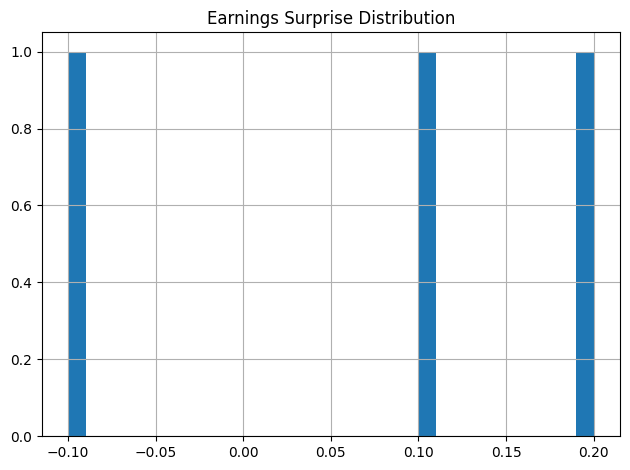
\includegraphics[keepaspectratio]{main_files/figure-pdf/cell-7-output-1.png}}

\begin{Shaded}
\begin{Highlighting}[]
\CommentTok{\# Identify highly correlated feature pairs}
\NormalTok{high\_corr\_threshold }\OperatorTok{=} \FloatTok{0.8}
\NormalTok{high\_corr\_pairs }\OperatorTok{=}\NormalTok{ []}
\ControlFlowTok{for}\NormalTok{ i }\KeywordTok{in} \BuiltInTok{range}\NormalTok{(}\BuiltInTok{len}\NormalTok{(correlation\_matrix)):}
    \ControlFlowTok{for}\NormalTok{ j }\KeywordTok{in} \BuiltInTok{range}\NormalTok{(i}\OperatorTok{+}\DecValTok{1}\NormalTok{, }\BuiltInTok{len}\NormalTok{(correlation\_matrix)):}
        \ControlFlowTok{if} \BuiltInTok{abs}\NormalTok{(correlation\_matrix.iloc[i, j]) }\OperatorTok{\textgreater{}}\NormalTok{ high\_corr\_threshold:}
\NormalTok{            high\_corr\_pairs.append((correlation\_matrix.index[i], }
\NormalTok{                                   correlation\_matrix.columns[j], }
\NormalTok{                                   correlation\_matrix.iloc[i, j]))}

\BuiltInTok{print}\NormalTok{(}\SpecialStringTok{f"}\CharTok{\textbackslash{}n}\SpecialStringTok{Highly correlated feature pairs (|r| \textgreater{} }\SpecialCharTok{\{}\NormalTok{high\_corr\_threshold}\SpecialCharTok{\}}\SpecialStringTok{):"}\NormalTok{)}
\ControlFlowTok{for}\NormalTok{ feat1, feat2, corr }\KeywordTok{in}\NormalTok{ high\_corr\_pairs[:}\DecValTok{5}\NormalTok{]:  }\CommentTok{\# Show top 5}
    \BuiltInTok{print}\NormalTok{(}\SpecialStringTok{f"  }\SpecialCharTok{\{}\NormalTok{feat1}\SpecialCharTok{\}}\SpecialStringTok{ ↔ }\SpecialCharTok{\{}\NormalTok{feat2}\SpecialCharTok{\}}\SpecialStringTok{: r = }\SpecialCharTok{\{}\NormalTok{corr}\SpecialCharTok{:.3f\}}\SpecialStringTok{"}\NormalTok{)}

\BuiltInTok{print}\NormalTok{(}\StringTok{"}\CharTok{\textbackslash{}n}\StringTok{Key Finding: High correlation between sensors measuring same chemical property"}\NormalTok{)}
\BuiltInTok{print}\NormalTok{(}\StringTok{"(e.g., steady{-}state features from same sensor show strong positive correlation)"}\NormalTok{)}
\end{Highlighting}
\end{Shaded}

\begin{verbatim}

Highly correlated feature pairs (|r| > 0.8):
  S01_F1_DR ↔ S01_F3_EMAi_001: r = 0.984
  S01_F1_DR ↔ S01_F4_EMAi_01: r = 0.964
  S01_F1_DR ↔ S01_F5_EMAi_1: r = 0.852
  S01_F1_DR ↔ S01_F6_EMAd_001: r = -0.951
  S01_F1_DR ↔ S01_F7_EMAd_01: r = -0.883

Key Finding: High correlation between sensors measuring same chemical property
(e.g., steady-state features from same sensor show strong positive correlation)
\end{verbatim}

\subsection{Temporal Drift Pattern
Analysis}\label{temporal-drift-pattern-analysis}

The dataset spans 10 batches over 36 months, providing a window into
sensor aging. This analysis tracks mean responses across batches for 4
sensors representing different feature types.

\textbf{Key Questions:} - Do responses shift consistently over time
(systematic drift vs.~random noise)? - Do different feature types drift
at different rates? - Does variability (std dev) change with aging?

Trend lines quantify drift velocity, providing the first direct
measurement of degradation rates in this sensor array.

\begin{Shaded}
\begin{Highlighting}[]
\CommentTok{\# Calculate mean responses per batch for selected sensors}
\NormalTok{temporal\_sensors }\OperatorTok{=}\NormalTok{ [}\StringTok{\textquotesingle{}S01\_F1\_DR\textquotesingle{}}\NormalTok{, }\StringTok{\textquotesingle{}S05\_F2\_DR\_norm\textquotesingle{}}\NormalTok{, }\StringTok{\textquotesingle{}S08\_F6\_EMAd\_001\textquotesingle{}}\NormalTok{, }\StringTok{\textquotesingle{}S12\_F4\_EMAi\_01\textquotesingle{}}\NormalTok{]}
\NormalTok{temporal\_data }\OperatorTok{=}\NormalTok{ []}

\NormalTok{batches }\OperatorTok{=} \BuiltInTok{sorted}\NormalTok{(df[}\StringTok{\textquotesingle{}batch\textquotesingle{}}\NormalTok{].unique())}
\ControlFlowTok{for}\NormalTok{ batch }\KeywordTok{in}\NormalTok{ batches:}
\NormalTok{    batch\_mask }\OperatorTok{=}\NormalTok{ df[}\StringTok{\textquotesingle{}batch\textquotesingle{}}\NormalTok{] }\OperatorTok{==}\NormalTok{ batch}
    \ControlFlowTok{for}\NormalTok{ sensor }\KeywordTok{in}\NormalTok{ temporal\_sensors:}
\NormalTok{        temporal\_data.append(\{}
            \StringTok{\textquotesingle{}batch\textquotesingle{}}\NormalTok{: batch,}
            \StringTok{\textquotesingle{}sensor\textquotesingle{}}\NormalTok{: sensor,}
            \StringTok{\textquotesingle{}mean\_response\textquotesingle{}}\NormalTok{: df[batch\_mask][sensor].mean(),}
            \StringTok{\textquotesingle{}std\_response\textquotesingle{}}\NormalTok{: df[batch\_mask][sensor].std()}
\NormalTok{        \})}

\NormalTok{temporal\_df }\OperatorTok{=}\NormalTok{ pd.DataFrame(temporal\_data)}
\end{Highlighting}
\end{Shaded}

\begin{Shaded}
\begin{Highlighting}[]
\CommentTok{\# Visualize temporal patterns}
\NormalTok{fig, axes }\OperatorTok{=}\NormalTok{ plt.subplots(}\DecValTok{2}\NormalTok{, }\DecValTok{2}\NormalTok{, figsize}\OperatorTok{=}\NormalTok{(}\DecValTok{15}\NormalTok{, }\DecValTok{10}\NormalTok{))}
\NormalTok{axes }\OperatorTok{=}\NormalTok{ axes.flatten()}

\ControlFlowTok{for}\NormalTok{ idx, sensor }\KeywordTok{in} \BuiltInTok{enumerate}\NormalTok{(temporal\_sensors):}
\NormalTok{    sensor\_data }\OperatorTok{=}\NormalTok{ temporal\_df[temporal\_df[}\StringTok{\textquotesingle{}sensor\textquotesingle{}}\NormalTok{] }\OperatorTok{==}\NormalTok{ sensor]}
    
\NormalTok{    axes[idx].errorbar(sensor\_data[}\StringTok{\textquotesingle{}batch\textquotesingle{}}\NormalTok{], sensor\_data[}\StringTok{\textquotesingle{}mean\_response\textquotesingle{}}\NormalTok{],}
\NormalTok{                       yerr}\OperatorTok{=}\NormalTok{sensor\_data[}\StringTok{\textquotesingle{}std\_response\textquotesingle{}}\NormalTok{], }
\NormalTok{                       marker}\OperatorTok{=}\StringTok{\textquotesingle{}o\textquotesingle{}}\NormalTok{, linewidth}\OperatorTok{=}\DecValTok{2}\NormalTok{, capsize}\OperatorTok{=}\DecValTok{5}\NormalTok{, capthick}\OperatorTok{=}\DecValTok{2}\NormalTok{)}
\NormalTok{    axes[idx].set\_xlabel(}\StringTok{\textquotesingle{}Batch Number\textquotesingle{}}\NormalTok{)}
\NormalTok{    axes[idx].set\_ylabel(}\StringTok{\textquotesingle{}Mean Sensor Response\textquotesingle{}}\NormalTok{)}
\NormalTok{    axes[idx].set\_title(}\SpecialStringTok{f\textquotesingle{}Temporal Evolution: }\SpecialCharTok{\{}\NormalTok{sensor}\SpecialCharTok{\}}\SpecialStringTok{\textquotesingle{}}\NormalTok{)}
\NormalTok{    axes[idx].grid(}\VariableTok{True}\NormalTok{, alpha}\OperatorTok{=}\FloatTok{0.3}\NormalTok{)}
    
    \CommentTok{\# Add trend line}
\NormalTok{    z }\OperatorTok{=}\NormalTok{ np.polyfit(sensor\_data[}\StringTok{\textquotesingle{}batch\textquotesingle{}}\NormalTok{], sensor\_data[}\StringTok{\textquotesingle{}mean\_response\textquotesingle{}}\NormalTok{], }\DecValTok{1}\NormalTok{)}
\NormalTok{    p }\OperatorTok{=}\NormalTok{ np.poly1d(z)}
\NormalTok{    axes[idx].plot(sensor\_data[}\StringTok{\textquotesingle{}batch\textquotesingle{}}\NormalTok{], p(sensor\_data[}\StringTok{\textquotesingle{}batch\textquotesingle{}}\NormalTok{]), }
                  \StringTok{\textquotesingle{}r{-}{-}\textquotesingle{}}\NormalTok{, alpha}\OperatorTok{=}\FloatTok{0.5}\NormalTok{, label}\OperatorTok{=}\SpecialStringTok{f\textquotesingle{}Trend: slope=}\SpecialCharTok{\{}\NormalTok{z[}\DecValTok{0}\NormalTok{]}\SpecialCharTok{:.3f\}}\SpecialStringTok{\textquotesingle{}}\NormalTok{)}
\NormalTok{    axes[idx].legend()}

\NormalTok{plt.suptitle(}\StringTok{\textquotesingle{}Temporal Drift Patterns Across Sensor Types\textquotesingle{}}\NormalTok{, fontsize}\OperatorTok{=}\DecValTok{14}\NormalTok{, y}\OperatorTok{=}\FloatTok{1.02}\NormalTok{)}
\NormalTok{plt.tight\_layout()}
\NormalTok{plt.show()}

\BuiltInTok{print}\NormalTok{(}\StringTok{"}\CharTok{\textbackslash{}n}\StringTok{Finding: Systematic drift visible in raw features across all sensor types"}\NormalTok{)}
\BuiltInTok{print}\NormalTok{(}\StringTok{"Different sensors show varying drift rates and directions"}\NormalTok{)}
\BuiltInTok{print}\NormalTok{(}\StringTok{"This motivates the need for PCA to find stable measurement modes"}\NormalTok{)}
\end{Highlighting}
\end{Shaded}

\pandocbounded{\includegraphics[keepaspectratio]{main_files/figure-pdf/cell-10-output-1.png}}

\begin{verbatim}

Finding: Systematic drift visible in raw features across all sensor types
Different sensors show varying drift rates and directions
This motivates the need for PCA to find stable measurement modes
\end{verbatim}

\subsection{Variance Analysis by Feature
Type}\label{variance-analysis-by-feature-type}

Building on the initial data inspection, we now perform detailed
statistical analysis of variance patterns across the 8 feature types.
This analysis quantifies variance distribution (mean, std, min, max) to
understand which measurement types contribute most to the signal and how
consistent sensors are within each type.

\begin{Shaded}
\begin{Highlighting}[]
\CommentTok{\# Group features by type based on naming convention}
\NormalTok{feature\_types }\OperatorTok{=}\NormalTok{ \{}
    \StringTok{\textquotesingle{}F1\_DR\textquotesingle{}}\NormalTok{: [],           }\CommentTok{\# Steady{-}state resistance}
    \StringTok{\textquotesingle{}F2\_DR\_norm\textquotesingle{}}\NormalTok{: [],      }\CommentTok{\# Normalized steady{-}state}
    \StringTok{\textquotesingle{}F3\_EMAi\_001\textquotesingle{}}\NormalTok{: [],     }\CommentTok{\# Exponential moving average}
    \StringTok{\textquotesingle{}F4\_EMAi\_01\textquotesingle{}}\NormalTok{: [],      }\CommentTok{\# EMA intermediate}
    \StringTok{\textquotesingle{}F5\_EMAi\_1\textquotesingle{}}\NormalTok{: [],       }\CommentTok{\# EMA fast}
    \StringTok{\textquotesingle{}F6\_EMAd\_001\textquotesingle{}}\NormalTok{: [],     }\CommentTok{\# EMA derivative slow}
    \StringTok{\textquotesingle{}F7\_EMAd\_01\textquotesingle{}}\NormalTok{: [],      }\CommentTok{\# EMA derivative medium}
    \StringTok{\textquotesingle{}F8\_EMAd\_1\textquotesingle{}}\NormalTok{: []        }\CommentTok{\# EMA derivative fast}
\NormalTok{\}}

\ControlFlowTok{for}\NormalTok{ col }\KeywordTok{in}\NormalTok{ sensor\_cols:}
    \ControlFlowTok{for}\NormalTok{ feat\_type }\KeywordTok{in}\NormalTok{ feature\_types.keys():}
        \ControlFlowTok{if}\NormalTok{ feat\_type }\KeywordTok{in}\NormalTok{ col:}
\NormalTok{            feature\_types[feat\_type].append(col)}
            \ControlFlowTok{break}

\CommentTok{\# Calculate variance statistics by type}
\NormalTok{variance\_stats }\OperatorTok{=}\NormalTok{ []}
\ControlFlowTok{for}\NormalTok{ feat\_type, features }\KeywordTok{in}\NormalTok{ feature\_types.items():}
    \ControlFlowTok{if}\NormalTok{ features:}
\NormalTok{        variances }\OperatorTok{=}\NormalTok{ df[features].var()}
\NormalTok{        variance\_stats.append(\{}
            \StringTok{\textquotesingle{}Feature Type\textquotesingle{}}\NormalTok{: feat\_type,}
            \StringTok{\textquotesingle{}Count\textquotesingle{}}\NormalTok{: }\BuiltInTok{len}\NormalTok{(features),}
            \StringTok{\textquotesingle{}Mean Variance\textquotesingle{}}\NormalTok{: variances.mean(),}
            \StringTok{\textquotesingle{}Std Variance\textquotesingle{}}\NormalTok{: variances.std(),}
            \StringTok{\textquotesingle{}Min Variance\textquotesingle{}}\NormalTok{: variances.}\BuiltInTok{min}\NormalTok{(),}
            \StringTok{\textquotesingle{}Max Variance\textquotesingle{}}\NormalTok{: variances.}\BuiltInTok{max}\NormalTok{()}
\NormalTok{        \})}

\NormalTok{variance\_df }\OperatorTok{=}\NormalTok{ pd.DataFrame(variance\_stats)}
\NormalTok{variance\_df }\OperatorTok{=}\NormalTok{ variance\_df.sort\_values(}\StringTok{\textquotesingle{}Mean Variance\textquotesingle{}}\NormalTok{, ascending}\OperatorTok{=}\VariableTok{False}\NormalTok{)}

\BuiltInTok{print}\NormalTok{(}\StringTok{"}\CharTok{\textbackslash{}n}\StringTok{Variance Statistics by Feature Type:"}\NormalTok{)}
\NormalTok{display(variance\_df)}
\end{Highlighting}
\end{Shaded}

\begin{verbatim}

Variance Statistics by Feature Type:
\end{verbatim}

\begin{longtable}[]{@{}lllllll@{}}
\toprule\noalign{}
& Feature Type & Count & Mean Variance & Std Variance & Min Variance &
Max Variance \\
\midrule\noalign{}
\endhead
\bottomrule\noalign{}
\endlastfoot
0 & F1\_DR & 16 & 9.553401e+08 & 1.597560e+09 & 4.449158e+06 &
4.878294e+09 \\
1 & F2\_DR\_norm & 16 & 5.892398e+03 & 1.770543e+04 & 2.652267e+00 &
6.981400e+04 \\
7 & F8\_EMAd\_1 & 16 & 4.186679e+03 & 7.618150e+03 & 1.738429e+01 &
2.490161e+04 \\
4 & F5\_EMAi\_1 & 16 & 1.238948e+03 & 2.984741e+03 & 2.272869e+01 &
1.220889e+04 \\
3 & F4\_EMAi\_01 & 16 & 1.882594e+02 & 1.951099e+02 & 4.874575e+00 &
6.199826e+02 \\
6 & F7\_EMAd\_01 & 16 & 1.044718e+02 & 1.495097e+02 & 8.368293e-01 &
4.538863e+02 \\
2 & F3\_EMAi\_001 & 16 & 6.900143e+01 & 1.012626e+02 & 5.253051e-01 &
3.101142e+02 \\
5 & F6\_EMAd\_001 & 16 & 3.346509e+01 & 4.826921e+01 & 2.794819e-01 &
1.620327e+02 \\
\end{longtable}

\subsection{Variance Distribution
Visualization}\label{variance-distribution-visualization}

The tabular statistics reveal a 6-order-of-magnitude variance range, but
visualization makes this scale difference immediately apparent. The
log-scale bar chart compares feature types side-by-side, while the
histogram shows the overall distribution across all 128 individual
sensors.

\textbf{Key Insight:}

The variance ratio between steady-state (F1\_DR) and transient features
(F3-F8) quantifies signal dominance - if one feature type has 1,000,000×
more variance, it will overwhelm principal components unless features
are normalized. This finding directly motivates our PCA approach and
explains why dimensionality reduction is effective despite 128 features.

\begin{Shaded}
\begin{Highlighting}[]
\CommentTok{\# Visualize variance distribution}
\NormalTok{fig, axes }\OperatorTok{=}\NormalTok{ plt.subplots(}\DecValTok{1}\NormalTok{, }\DecValTok{2}\NormalTok{, figsize}\OperatorTok{=}\NormalTok{(}\DecValTok{15}\NormalTok{, }\DecValTok{5}\NormalTok{))}

\CommentTok{\# Bar plot of mean variance by type}
\NormalTok{axes[}\DecValTok{0}\NormalTok{].bar(}\BuiltInTok{range}\NormalTok{(}\BuiltInTok{len}\NormalTok{(variance\_df)), variance\_df[}\StringTok{\textquotesingle{}Mean Variance\textquotesingle{}}\NormalTok{], }
\NormalTok{           color}\OperatorTok{=}\StringTok{\textquotesingle{}steelblue\textquotesingle{}}\NormalTok{, alpha}\OperatorTok{=}\FloatTok{0.7}\NormalTok{)}
\NormalTok{axes[}\DecValTok{0}\NormalTok{].set\_xticks(}\BuiltInTok{range}\NormalTok{(}\BuiltInTok{len}\NormalTok{(variance\_df)))}
\NormalTok{axes[}\DecValTok{0}\NormalTok{].set\_xticklabels(variance\_df[}\StringTok{\textquotesingle{}Feature Type\textquotesingle{}}\NormalTok{], rotation}\OperatorTok{=}\DecValTok{45}\NormalTok{, ha}\OperatorTok{=}\StringTok{\textquotesingle{}right\textquotesingle{}}\NormalTok{)}
\NormalTok{axes[}\DecValTok{0}\NormalTok{].set\_ylabel(}\StringTok{\textquotesingle{}Mean Variance (log scale)\textquotesingle{}}\NormalTok{)}
\NormalTok{axes[}\DecValTok{0}\NormalTok{].set\_yscale(}\StringTok{\textquotesingle{}log\textquotesingle{}}\NormalTok{)}
\NormalTok{axes[}\DecValTok{0}\NormalTok{].set\_title(}\StringTok{\textquotesingle{}Variance by Feature Type\textquotesingle{}}\NormalTok{)}
\NormalTok{axes[}\DecValTok{0}\NormalTok{].grid(}\VariableTok{True}\NormalTok{, alpha}\OperatorTok{=}\FloatTok{0.3}\NormalTok{)}

\CommentTok{\# Variance distribution across all features}
\NormalTok{all\_variances }\OperatorTok{=}\NormalTok{ df[sensor\_cols].var()}
\NormalTok{axes[}\DecValTok{1}\NormalTok{].hist(np.log10(all\_variances), bins}\OperatorTok{=}\DecValTok{30}\NormalTok{, edgecolor}\OperatorTok{=}\StringTok{\textquotesingle{}black\textquotesingle{}}\NormalTok{, alpha}\OperatorTok{=}\FloatTok{0.7}\NormalTok{)}
\NormalTok{axes[}\DecValTok{1}\NormalTok{].set\_xlabel(}\StringTok{\textquotesingle{}Log10(Variance)\textquotesingle{}}\NormalTok{)}
\NormalTok{axes[}\DecValTok{1}\NormalTok{].set\_ylabel(}\StringTok{\textquotesingle{}Number of Features\textquotesingle{}}\NormalTok{)}
\NormalTok{axes[}\DecValTok{1}\NormalTok{].set\_title(}\StringTok{\textquotesingle{}Distribution of Feature Variances\textquotesingle{}}\NormalTok{)}
\NormalTok{axes[}\DecValTok{1}\NormalTok{].grid(}\VariableTok{True}\NormalTok{, alpha}\OperatorTok{=}\FloatTok{0.3}\NormalTok{)}

\NormalTok{plt.tight\_layout()}
\NormalTok{plt.show()}

\CommentTok{\# Calculate variance ratio}
\NormalTok{f1\_mask }\OperatorTok{=}\NormalTok{ variance\_df[}\StringTok{\textquotesingle{}Feature Type\textquotesingle{}}\NormalTok{] }\OperatorTok{==} \StringTok{\textquotesingle{}F1\_DR\textquotesingle{}}
\NormalTok{f1\_variance }\OperatorTok{=}\NormalTok{ variance\_df[f1\_mask][}\StringTok{\textquotesingle{}Mean Variance\textquotesingle{}}\NormalTok{].values[}\DecValTok{0}\NormalTok{]}

\NormalTok{ema\_mask }\OperatorTok{=}\NormalTok{ variance\_df[}\StringTok{\textquotesingle{}Feature Type\textquotesingle{}}\NormalTok{].}\BuiltInTok{str}\NormalTok{.contains(}\StringTok{\textquotesingle{}EMA\textquotesingle{}}\NormalTok{)}
\NormalTok{transient\_variance }\OperatorTok{=}\NormalTok{ variance\_df[ema\_mask][}\StringTok{\textquotesingle{}Mean Variance\textquotesingle{}}\NormalTok{].mean()}

\NormalTok{variance\_ratio }\OperatorTok{=}\NormalTok{ f1\_variance }\OperatorTok{/}\NormalTok{ transient\_variance}

\BuiltInTok{print}\NormalTok{(}\SpecialStringTok{f"}\CharTok{\textbackslash{}n}\SpecialStringTok{Key Finding: F1 (DR) features have }\SpecialCharTok{\{}\NormalTok{variance\_ratio}\SpecialCharTok{:.0f\}}\SpecialStringTok{x "}
      \SpecialStringTok{f"more variance than transient features."}\NormalTok{)}
\BuiltInTok{print}\NormalTok{(}\StringTok{"This suggests steady{-}state signals dominate over transient features"}\NormalTok{)}
\end{Highlighting}
\end{Shaded}

\pandocbounded{\includegraphics[keepaspectratio]{main_files/figure-pdf/cell-12-output-1.png}}

\begin{verbatim}

Key Finding: F1 (DR) features have 984747x more variance than transient features.
This suggests steady-state signals dominate over transient features
\end{verbatim}

\subsection{EDA Chapter Summary}\label{eda-chapter-summary}

The Exploratory Data Analysis chapter revealed distinct sensor response
patterns for each gas type, confirming that chemical fingerprints exist
in the data. Correlation analysis uncovered substantial linear structure
with mean pairwise correlation of 0.34, while within-sensor measurements
showed strong correlations exceeding 0.8. This linear structure
validates PCA's core assumption that important patterns can be captured
through linear combinations.

Temporal drift analysis demonstrated that sensor degradation follows
systematic patterns rather than random noise, with different sensors
showing varying drift rates and directions. The variance analysis
quantified a remarkable 6-order-of-magnitude range across features, with
steady-state F1 features showing 984,747× more variance than transient
features. This extreme variance hierarchy explains why PCA can
effectively compress the data from 128 dimensions to just 8 while
retaining 90\% of the information. The clean data quality enabled the
project to focus on sophisticated drift analysis rather than extensive
preprocessing, while the discovered variance structure and temporal
patterns directly motivated the choice of PCA as the primary analytical
method.

\section{PCA-Based Drift Analysis}\label{pca-based-drift-analysis}

This section introduces our analytical framework for understanding
sensor drift through geometric analysis. We employ two primary
unsupervised learning techniques: \textbf{Principal Component Analysis
(PCA)} for dimensionality reduction and drift pattern discovery, and
\textbf{K-means clustering} for validating that chemical signatures
remain distinguishable despite temporal degradation.

\subsection{Why PCA? Model Selection
Justification}\label{why-pca-model-selection-justification}

\subsubsection{PCA Assumptions - Validated by
EDA}\label{pca-assumptions---validated-by-eda}

\textbf{Linear Relationships Assumption}: PCA assumes that important
patterns can be captured through linear combinations of features. Our
EDA correlation analysis validated this assumption, showing mean
pairwise correlation \textbar r\textbar{} = 0.34 across the first 30
features, with strong within-sensor correlations (\textgreater0.8 for
related measurements like F1\_DR with F3-F5\_EMAi), confirming
substantial linear structure exists in the 128-dimensional sensor space.

\textbf{High-Variance = High-Information Assumption}: PCA assumes
directions of maximum variance contain the most signal. For sensor drift
analysis, this is appropriate because: (1) EDA variance analysis
revealed a 6 order of magnitude range across features, and (2) temporal
analysis showed drift follows structured patterns rather than random
noise---creating high variance when pooling across batches.

\subsubsection{Why Not Alternative Dimensionality Reduction
Methods?}\label{why-not-alternative-dimensionality-reduction-methods}

\textbf{t-SNE/UMAP}: While excellent for visualization, these methods
lack the interpretability needed for stability analysis. Embeddings
change with each run, preventing meaningful temporal drift tracking
across batches.

\textbf{Autoencoders}: More powerful for capturing nonlinear
relationships but introduce many hyperparameters and lack PCA's
closed-form eigenvalue decomposition. The interpretability vs.~power
trade-off favors PCA for geometric drift analysis, where we need to
precisely measure how principal directions change over time.

\textbf{ICA (Independent Component Analysis)}: Seeks statistically
independent components rather than orthogonal variance-maximizing
directions. While valuable for blind source separation, our goal is
finding stable variance directions, making PCA's variance-based
decomposition more appropriate.

\subsubsection{Why K-means? Clustering Validation
Justification}\label{why-k-means-clustering-validation-justification}

K-means clustering serves as our validation tool to verify that chemical
signatures remain distinguishable despite drift. We use clustering
quality metrics (silhouette score, Davies-Bouldin index,
Calinski-Harabasz score) across different PC subspaces to assess drift
resistance.

\subsubsection{K-means Assumptions - Supported by
EDA}\label{k-means-assumptions---supported-by-eda}

\textbf{Spherical Cluster Assumption}: K-means assumes clusters are
roughly spherical in the feature space. While we cannot fully validate
this until after dimensionality reduction, the moderate correlations
observed in EDA (\textbar r\textbar=0.34) suggest cluster shapes should
be reasonably regular.

\textbf{Known Number of Clusters (k=6)}: We know a priori that 6
chemical classes exist, confirmed by EDA showing 6 distinct gas types
with adequate sample sizes. We validate this choice using elbow analysis
and silhouette scores.

\textbf{Balanced Cluster Sizes}: K-means can struggle with severely
imbalanced clusters. Our EDA showed acceptable class balance with
1,641-3,009 samples per gas type (1.83:1 ratio), well within K-means'
operating range.

\subsubsection{Why K-means as Primary Validation
Tool?}\label{why-k-means-as-primary-validation-tool}

\textbf{DBSCAN}: While we test DBSCAN for robustness, it requires
careful epsilon tuning and can struggle with varying cluster densities
across batches, making it less suitable as our primary validation
metric.

\textbf{Hierarchical Clustering}: We also test hierarchical clustering
for comparison, but K-means' simplicity and well-defined optimization
objective make it ideal for primary validation metrics. Consistency
across multiple algorithms strengthens our conclusions.

\subsubsection{Analytical Framework}\label{analytical-framework}

Our analysis combines PCA and K-means in a complementary way:

\begin{enumerate}
\def\labelenumi{\arabic{enumi}.}
\tightlist
\item
  \textbf{PCA discovers structure}: We identify the intrinsic
  dimensionality, reveal which directions drift most/least, and
  characterize drift as geometric transformations
\item
  \textbf{K-means validates discriminability}: We confirm that chemical
  signatures remain separable in different PC subspaces despite temporal
  drift
\item
  \textbf{Multi-algorithm robustness}: Testing multiple clustering
  algorithms ensures our findings aren't artifacts of a single method
\end{enumerate}

\subsubsection{Conclusion}\label{conclusion}

PCA is optimal for drift discovery because EDA confirmed: (1)
substantial linear structure exists in the data, (2) high-variance
directions capture systematic drift patterns, and (3) the closed-form
eigenvalue solution enables precise geometric measurement while
maintaining interpretability.

K-means is optimal for validation because: (1) we know the true number
of classes, (2) EDA confirmed balanced class distributions, and (3) its
simplicity provides stable, interpretable quality metrics.

Together, these methods form a rigorous unsupervised framework for
discovering and validating drift-resistant feature representations.

\subsection{Setup for Analysis}\label{setup-for-analysis}

\subsubsection{Mathematical Framework}\label{mathematical-framework}

\textbf{PCA Formulation}: Given standardized sensor data matrix
\textbf{X} ∈ ℝⁿˣ¹²⁸ (n samples, 128 features), PCA finds orthogonal
directions of maximum variance by solving the eigenvalue problem:

\textbf{Σv} = λ\textbf{v}

where \textbf{Σ} = (1/n)\textbf{X}ᵀ\textbf{X} is the covariance matrix,
\textbf{v} are eigenvectors (principal components), and λ are
eigenvalues. The variance explained by PC\_i is:

Variance explained ratio\_i = λᵢ / Σⱼλⱼ

We order components by decreasing eigenvalue: λ₁ ≥ λ₂ ≥ \ldots{} ≥ λ₁₂₈.

\textbf{Stability Metric Definition}: To measure temporal stability of
principal components, we define the \emph{centroid drift magnitude} for
PC\_i across consecutive batches:

Drift\_i = Σₜ \textbar\textbar μᵢ(t+1) - μᵢ(t)\textbar\textbar₂

where μᵢ(t) is the centroid (mean) of PC\_i scores in batch t, and
\textbar\textbar·\textbar\textbar₂ is the Euclidean norm. Lower drift
indicates more stable components.

\textbf{Clustering Quality Metrics}: We use three complementary metrics:

\begin{itemize}
\item
  \textbf{Silhouette score}: s = (b - a) / max(a, b), where a = mean
  intra-cluster distance, b = mean nearest-cluster distance. Range
  {[}-1, 1{]}, higher is better.
\item
  \textbf{Davies-Bouldin index}: DB = (1/k) Σᵢ max\_j≠i {[}(σᵢ + σⱼ) /
  d(cᵢ, cⱼ){]}, where σᵢ is cluster scatter, d(cᵢ, cⱼ) is centroid
  distance. Lower is better.
\item
  \textbf{Calinski-Harabasz score}: CH = {[}tr(B\_k) / (k-1){]} /
  {[}tr(W\_k) / (n-k){]}, where B\_k is between-cluster scatter, W\_k is
  within-cluster scatter. Higher is better.
\end{itemize}

\begin{Shaded}
\begin{Highlighting}[]
\CommentTok{\# Additional imports for PCA analysis}
\ImportTok{from}\NormalTok{ scipy.spatial.distance }\ImportTok{import}\NormalTok{ cdist, pdist}
\ImportTok{from}\NormalTok{ scipy.optimize }\ImportTok{import}\NormalTok{ linear\_sum\_assignment}
\ImportTok{from}\NormalTok{ scipy.stats }\ImportTok{import}\NormalTok{ spearmanr}
\ImportTok{from}\NormalTok{ scipy.linalg }\ImportTok{import}\NormalTok{ orthogonal\_procrustes, subspace\_angles}
\ImportTok{from}\NormalTok{ sklearn.decomposition }\ImportTok{import}\NormalTok{ PCA}
\ImportTok{from}\NormalTok{ sklearn.preprocessing }\ImportTok{import}\NormalTok{ StandardScaler}
\ImportTok{from}\NormalTok{ sklearn.cluster }\ImportTok{import}\NormalTok{ KMeans, DBSCAN, AgglomerativeClustering}
\ImportTok{from}\NormalTok{ sklearn.metrics }\ImportTok{import}\NormalTok{ silhouette\_score, davies\_bouldin\_score, calinski\_harabasz\_score}
\ImportTok{from}\NormalTok{ sklearn.neighbors }\ImportTok{import}\NormalTok{ NearestNeighbors}
\ImportTok{from}\NormalTok{ IPython.display }\ImportTok{import}\NormalTok{ display}

\CommentTok{\# Extract sensor columns and batches}
\NormalTok{sensor\_cols }\OperatorTok{=}\NormalTok{ [col }\ControlFlowTok{for}\NormalTok{ col }\KeywordTok{in}\NormalTok{ df.columns }\ControlFlowTok{if}\NormalTok{ col.startswith(}\StringTok{"S"}\NormalTok{)]}
\NormalTok{batches }\OperatorTok{=} \BuiltInTok{sorted}\NormalTok{(df[}\StringTok{"batch"}\NormalTok{].unique())}

\CommentTok{\# Standardize sensor readings}
\NormalTok{scaler }\OperatorTok{=}\NormalTok{ StandardScaler()}
\NormalTok{X\_scaled }\OperatorTok{=}\NormalTok{ scaler.fit\_transform(df[sensor\_cols])}

\BuiltInTok{print}\NormalTok{(}\SpecialStringTok{f"Data prepared for PCA: }\SpecialCharTok{\{}\NormalTok{X\_scaled}\SpecialCharTok{.}\NormalTok{shape[}\DecValTok{0}\NormalTok{]}\SpecialCharTok{\}}\SpecialStringTok{ samples, }\SpecialCharTok{\{}\NormalTok{X\_scaled}\SpecialCharTok{.}\NormalTok{shape[}\DecValTok{1}\NormalTok{]}\SpecialCharTok{\}}\SpecialStringTok{ sensors, }\SpecialCharTok{\{}\BuiltInTok{len}\NormalTok{(batches)}\SpecialCharTok{\}}\SpecialStringTok{ batches"}\NormalTok{)}
\BuiltInTok{print}\NormalTok{(}\SpecialStringTok{f"Time span: Batch }\SpecialCharTok{\{}\NormalTok{batches[}\DecValTok{0}\NormalTok{]}\SpecialCharTok{\}}\SpecialStringTok{ to Batch }\SpecialCharTok{\{}\NormalTok{batches[}\OperatorTok{{-}}\DecValTok{1}\NormalTok{]}\SpecialCharTok{\}}\SpecialStringTok{"}\NormalTok{)}
\end{Highlighting}
\end{Shaded}

\begin{verbatim}
Data prepared for PCA: 13910 samples, 128 sensors, 10 batches
Time span: Batch 1 to Batch 10
\end{verbatim}

\subsection{Dimensionality Discovery}\label{dimensionality-discovery}

First, we investigate the intrinsic dimensionality of the sensor array
data through eigenvalue spectrum analysis.

\begin{Shaded}
\begin{Highlighting}[]
\CommentTok{\# Perform global PCA}
\NormalTok{pca\_global }\OperatorTok{=}\NormalTok{ PCA(n\_components}\OperatorTok{=}\DecValTok{30}\NormalTok{, svd\_solver}\OperatorTok{=}\StringTok{\textquotesingle{}full\textquotesingle{}}\NormalTok{)}
\NormalTok{scores\_global }\OperatorTok{=}\NormalTok{ pca\_global.fit\_transform(X\_scaled)}

\CommentTok{\# Create explained variance dataframe}
\NormalTok{explained\_df }\OperatorTok{=}\NormalTok{ pd.DataFrame(\{}
    \StringTok{"component"}\NormalTok{: np.arange(}\DecValTok{1}\NormalTok{, pca\_global.n\_components\_ }\OperatorTok{+} \DecValTok{1}\NormalTok{),}
    \StringTok{"explained\_variance\_ratio"}\NormalTok{: pca\_global.explained\_variance\_ratio\_,}
    \StringTok{"eigenvalue"}\NormalTok{: pca\_global.explained\_variance\_}
\NormalTok{\})}
\NormalTok{explained\_df[}\StringTok{"cumulative\_variance"}\NormalTok{] }\OperatorTok{=}\NormalTok{ explained\_df[}\StringTok{"explained\_variance\_ratio"}\NormalTok{].cumsum()}

\BuiltInTok{print}\NormalTok{(}\StringTok{"}\CharTok{\textbackslash{}n}\StringTok{Variance explained by principal components:"}\NormalTok{)}
\NormalTok{display(explained\_df.head(}\DecValTok{12}\NormalTok{))}
\end{Highlighting}
\end{Shaded}

\begin{verbatim}

Variance explained by principal components:
\end{verbatim}

\begin{longtable}[]{@{}lllll@{}}
\toprule\noalign{}
& component & explained\_variance\_ratio & eigenvalue &
cumulative\_variance \\
\midrule\noalign{}
\endhead
\bottomrule\noalign{}
\endlastfoot
0 & 1 & 0.535151 & 68.504298 & 0.535151 \\
1 & 2 & 0.150401 & 19.252659 & 0.685552 \\
2 & 3 & 0.060458 & 7.739124 & 0.746009 \\
3 & 4 & 0.050850 & 6.509256 & 0.796859 \\
4 & 5 & 0.035277 & 4.515747 & 0.832136 \\
5 & 6 & 0.029060 & 3.719978 & 0.861196 \\
6 & 7 & 0.023333 & 2.986861 & 0.884530 \\
7 & 8 & 0.015695 & 2.009168 & 0.900225 \\
8 & 9 & 0.014492 & 1.855114 & 0.914717 \\
9 & 10 & 0.011713 & 1.499318 & 0.926430 \\
10 & 11 & 0.010263 & 1.313760 & 0.936693 \\
11 & 12 & 0.008979 & 1.149364 & 0.945671 \\
\end{longtable}

\subsection{Dimensionality
Visualization}\label{dimensionality-visualization}

\begin{Shaded}
\begin{Highlighting}[]
\CommentTok{\# Visualization}
\NormalTok{fig, axes }\OperatorTok{=}\NormalTok{ plt.subplots(}\DecValTok{1}\NormalTok{, }\DecValTok{3}\NormalTok{, figsize}\OperatorTok{=}\NormalTok{(}\DecValTok{15}\NormalTok{, }\DecValTok{4}\NormalTok{))}

\CommentTok{\# Scree plot}
\NormalTok{axes[}\DecValTok{0}\NormalTok{].plot(explained\_df[}\StringTok{\textquotesingle{}component\textquotesingle{}}\NormalTok{], explained\_df[}\StringTok{\textquotesingle{}eigenvalue\textquotesingle{}}\NormalTok{], }\StringTok{\textquotesingle{}o{-}\textquotesingle{}}\NormalTok{)}
\CommentTok{\# Add Kaiser criterion with count}
\NormalTok{eigenvalues }\OperatorTok{=}\NormalTok{ pca\_global.explained\_variance\_}
\NormalTok{kaiser\_threshold }\OperatorTok{=}\NormalTok{ eigenvalues[eigenvalues }\OperatorTok{\textgreater{}} \DecValTok{1}\NormalTok{]}
\NormalTok{axes[}\DecValTok{0}\NormalTok{].axhline(y}\OperatorTok{=}\DecValTok{1}\NormalTok{, color}\OperatorTok{=}\StringTok{\textquotesingle{}r\textquotesingle{}}\NormalTok{, linestyle}\OperatorTok{=}\StringTok{\textquotesingle{}{-}{-}\textquotesingle{}}\NormalTok{, alpha}\OperatorTok{=}\FloatTok{0.5}\NormalTok{, }
\NormalTok{                label}\OperatorTok{=}\SpecialStringTok{f\textquotesingle{}Kaiser criterion (λ\textgreater{}1): }\SpecialCharTok{\{}\BuiltInTok{len}\NormalTok{(kaiser\_threshold)}\SpecialCharTok{\}}\SpecialStringTok{ PCs\textquotesingle{}}\NormalTok{)}
\NormalTok{axes[}\DecValTok{0}\NormalTok{].set\_xlabel(}\StringTok{\textquotesingle{}Principal Component\textquotesingle{}}\NormalTok{)}
\NormalTok{axes[}\DecValTok{0}\NormalTok{].set\_ylabel(}\StringTok{\textquotesingle{}Eigenvalue\textquotesingle{}}\NormalTok{)}
\NormalTok{axes[}\DecValTok{0}\NormalTok{].set\_title(}\StringTok{\textquotesingle{}Scree Plot\textquotesingle{}}\NormalTok{)}
\NormalTok{axes[}\DecValTok{0}\NormalTok{].legend()}
\NormalTok{axes[}\DecValTok{0}\NormalTok{].grid(}\VariableTok{True}\NormalTok{, alpha}\OperatorTok{=}\FloatTok{0.3}\NormalTok{)}

\CommentTok{\# Explained variance ratio}
\NormalTok{axes[}\DecValTok{1}\NormalTok{].bar(explained\_df[}\StringTok{\textquotesingle{}component\textquotesingle{}}\NormalTok{][:}\DecValTok{10}\NormalTok{], explained\_df[}\StringTok{\textquotesingle{}explained\_variance\_ratio\textquotesingle{}}\NormalTok{][:}\DecValTok{10}\NormalTok{])}
\NormalTok{axes[}\DecValTok{1}\NormalTok{].set\_xlabel(}\StringTok{\textquotesingle{}Principal Component\textquotesingle{}}\NormalTok{)}
\NormalTok{axes[}\DecValTok{1}\NormalTok{].set\_ylabel(}\StringTok{\textquotesingle{}Explained Variance Ratio\textquotesingle{}}\NormalTok{)}
\NormalTok{axes[}\DecValTok{1}\NormalTok{].set\_title(}\StringTok{\textquotesingle{}Variance Contribution per Component\textquotesingle{}}\NormalTok{)}
\NormalTok{axes[}\DecValTok{1}\NormalTok{].grid(}\VariableTok{True}\NormalTok{, alpha}\OperatorTok{=}\FloatTok{0.3}\NormalTok{)}

\CommentTok{\# Cumulative variance}
\NormalTok{axes[}\DecValTok{2}\NormalTok{].plot(explained\_df[}\StringTok{\textquotesingle{}component\textquotesingle{}}\NormalTok{], explained\_df[}\StringTok{\textquotesingle{}cumulative\_variance\textquotesingle{}}\NormalTok{], }\StringTok{\textquotesingle{}o{-}\textquotesingle{}}\NormalTok{)}
\NormalTok{axes[}\DecValTok{2}\NormalTok{].axhline(y}\OperatorTok{=}\FloatTok{0.95}\NormalTok{, color}\OperatorTok{=}\StringTok{\textquotesingle{}r\textquotesingle{}}\NormalTok{, linestyle}\OperatorTok{=}\StringTok{\textquotesingle{}{-}{-}\textquotesingle{}}\NormalTok{, alpha}\OperatorTok{=}\FloatTok{0.5}\NormalTok{, label}\OperatorTok{=}\StringTok{\textquotesingle{}95\% threshold\textquotesingle{}}\NormalTok{)}
\NormalTok{axes[}\DecValTok{2}\NormalTok{].axhline(y}\OperatorTok{=}\FloatTok{0.90}\NormalTok{, color}\OperatorTok{=}\StringTok{\textquotesingle{}orange\textquotesingle{}}\NormalTok{, linestyle}\OperatorTok{=}\StringTok{\textquotesingle{}{-}{-}\textquotesingle{}}\NormalTok{, alpha}\OperatorTok{=}\FloatTok{0.5}\NormalTok{, label}\OperatorTok{=}\StringTok{\textquotesingle{}90\% threshold\textquotesingle{}}\NormalTok{)}
\NormalTok{axes[}\DecValTok{2}\NormalTok{].set\_xlabel(}\StringTok{\textquotesingle{}Principal Component\textquotesingle{}}\NormalTok{)}
\NormalTok{axes[}\DecValTok{2}\NormalTok{].set\_ylabel(}\StringTok{\textquotesingle{}Cumulative Explained Variance\textquotesingle{}}\NormalTok{)}
\NormalTok{axes[}\DecValTok{2}\NormalTok{].set\_title(}\StringTok{\textquotesingle{}Cumulative Variance Explained\textquotesingle{}}\NormalTok{)}
\NormalTok{axes[}\DecValTok{2}\NormalTok{].legend()}
\NormalTok{axes[}\DecValTok{2}\NormalTok{].grid(}\VariableTok{True}\NormalTok{, alpha}\OperatorTok{=}\FloatTok{0.3}\NormalTok{)}

\NormalTok{plt.tight\_layout()}
\NormalTok{plt.show()}

\CommentTok{\# Key findings}
\NormalTok{n\_95 }\OperatorTok{=}\NormalTok{ (explained\_df[}\StringTok{\textquotesingle{}cumulative\_variance\textquotesingle{}}\NormalTok{] }\OperatorTok{\textgreater{}=} \FloatTok{0.95}\NormalTok{).idxmax() }\OperatorTok{+} \DecValTok{1}
\NormalTok{n\_90 }\OperatorTok{=}\NormalTok{ (explained\_df[}\StringTok{\textquotesingle{}cumulative\_variance\textquotesingle{}}\NormalTok{] }\OperatorTok{\textgreater{}=} \FloatTok{0.90}\NormalTok{).idxmax() }\OperatorTok{+} \DecValTok{1}
\BuiltInTok{print}\NormalTok{(}\SpecialStringTok{f"}\CharTok{\textbackslash{}n}\SpecialStringTok{Key Findings:"}\NormalTok{)}
\BuiltInTok{print}\NormalTok{(}\SpecialStringTok{f"{-} }\SpecialCharTok{\{}\NormalTok{n\_90}\SpecialCharTok{\}}\SpecialStringTok{ components explain 90\% of variance"}\NormalTok{)}
\BuiltInTok{print}\NormalTok{(}\SpecialStringTok{f"{-} }\SpecialCharTok{\{}\NormalTok{n\_95}\SpecialCharTok{\}}\SpecialStringTok{ components explain 95\% of variance"}\NormalTok{)}
\BuiltInTok{print}\NormalTok{(}\SpecialStringTok{f"{-} Conclusion: Dataset lives in \textasciitilde{}}\SpecialCharTok{\{}\NormalTok{n\_90}\SpecialCharTok{\}}\SpecialStringTok{D subspace, not 128D"}\NormalTok{)}
\end{Highlighting}
\end{Shaded}

\pandocbounded{\includegraphics[keepaspectratio]{main_files/figure-pdf/cell-15-output-1.png}}

\begin{verbatim}

Key Findings:
- 8 components explain 90% of variance
- 13 components explain 95% of variance
- Conclusion: Dataset lives in ~8D subspace, not 128D
\end{verbatim}

\subsection{Principal Component Stability
Analysis}\label{principal-component-stability-analysis}

We analyze drift patterns by tracking how batch centroids shift within
the global PC space over time.

\begin{Shaded}
\begin{Highlighting}[]
\CommentTok{\# Use global PCA scores for all batches (already computed in Section 1)}
\NormalTok{n\_pcs }\OperatorTok{=} \DecValTok{10}
\NormalTok{global\_scores\_subset }\OperatorTok{=}\NormalTok{ scores\_global[:, :n\_pcs]}

\CommentTok{\# Reference batch for comparison}
\NormalTok{reference\_batch }\OperatorTok{=}\NormalTok{ batches[}\DecValTok{0}\NormalTok{]}
\NormalTok{ref\_mask }\OperatorTok{=}\NormalTok{ df[}\StringTok{\textquotesingle{}batch\textquotesingle{}}\NormalTok{] }\OperatorTok{==}\NormalTok{ reference\_batch}
\NormalTok{ref\_centroid }\OperatorTok{=}\NormalTok{ global\_scores\_subset[ref\_mask].mean(axis}\OperatorTok{=}\DecValTok{0}\NormalTok{)}
\NormalTok{ref\_cov }\OperatorTok{=}\NormalTok{ np.cov(global\_scores\_subset[ref\_mask].T)}

\CommentTok{\# Measure stability metrics for each batch}
\NormalTok{stability\_metrics }\OperatorTok{=}\NormalTok{ []}

\ControlFlowTok{for}\NormalTok{ batch }\KeywordTok{in}\NormalTok{ batches:}
\NormalTok{    mask }\OperatorTok{=}\NormalTok{ df[}\StringTok{\textquotesingle{}batch\textquotesingle{}}\NormalTok{] }\OperatorTok{==}\NormalTok{ batch}
\NormalTok{    batch\_scores }\OperatorTok{=}\NormalTok{ global\_scores\_subset[mask]}
\NormalTok{    batch\_centroid }\OperatorTok{=}\NormalTok{ batch\_scores.mean(axis}\OperatorTok{=}\DecValTok{0}\NormalTok{)}
\NormalTok{    batch\_cov }\OperatorTok{=}\NormalTok{ np.cov(batch\_scores.T)}
    
    \CommentTok{\# Measure centroid shift per PC}
\NormalTok{    centroid\_shifts }\OperatorTok{=}\NormalTok{ batch\_centroid }\OperatorTok{{-}}\NormalTok{ ref\_centroid}
    
    \CommentTok{\# Measure covariance change (stability of variance structure)}
\NormalTok{    cov\_distance }\OperatorTok{=}\NormalTok{ np.linalg.norm(batch\_cov }\OperatorTok{{-}}\NormalTok{ ref\_cov, }\StringTok{\textquotesingle{}fro\textquotesingle{}}\NormalTok{)}
    
    \CommentTok{\# Store metrics for each PC}
    \ControlFlowTok{for}\NormalTok{ pc\_idx }\KeywordTok{in} \BuiltInTok{range}\NormalTok{(n\_pcs):}
\NormalTok{        stability\_metrics.append(\{}
            \StringTok{\textquotesingle{}batch\textquotesingle{}}\NormalTok{: batch,}
            \StringTok{\textquotesingle{}PC\textquotesingle{}}\NormalTok{: pc\_idx }\OperatorTok{+} \DecValTok{1}\NormalTok{,}
            \StringTok{\textquotesingle{}centroid\_shift\textquotesingle{}}\NormalTok{: }\BuiltInTok{abs}\NormalTok{(centroid\_shifts[pc\_idx]),}
            \StringTok{\textquotesingle{}centroid\_shift\_signed\textquotesingle{}}\NormalTok{: centroid\_shifts[pc\_idx],}
            \StringTok{\textquotesingle{}variance\_explained\textquotesingle{}}\NormalTok{: pca\_global.explained\_variance\_ratio\_[pc\_idx],}
            \StringTok{\textquotesingle{}cov\_distance\textquotesingle{}}\NormalTok{: cov\_distance }\ControlFlowTok{if}\NormalTok{ batch }\OperatorTok{!=}\NormalTok{ reference\_batch }\ControlFlowTok{else} \DecValTok{0}
\NormalTok{        \})}

\NormalTok{stability\_df }\OperatorTok{=}\NormalTok{ pd.DataFrame(stability\_metrics)}
\end{Highlighting}
\end{Shaded}

\begin{Shaded}
\begin{Highlighting}[]
\NormalTok{fig, axes }\OperatorTok{=}\NormalTok{ plt.subplots(}\DecValTok{1}\NormalTok{, }\DecValTok{3}\NormalTok{, figsize}\OperatorTok{=}\NormalTok{(}\DecValTok{18}\NormalTok{, }\DecValTok{5}\NormalTok{))}

\CommentTok{\# 1. Centroid shifts over time}
\NormalTok{pivot\_shifts }\OperatorTok{=}\NormalTok{ stability\_df.pivot(index}\OperatorTok{=}\StringTok{\textquotesingle{}batch\textquotesingle{}}\NormalTok{, columns}\OperatorTok{=}\StringTok{\textquotesingle{}PC\textquotesingle{}}\NormalTok{, values}\OperatorTok{=}\StringTok{\textquotesingle{}centroid\_shift\textquotesingle{}}\NormalTok{)}
\ControlFlowTok{for}\NormalTok{ pc }\KeywordTok{in} \BuiltInTok{range}\NormalTok{(}\DecValTok{1}\NormalTok{, }\BuiltInTok{min}\NormalTok{(}\DecValTok{6}\NormalTok{, n\_pcs}\OperatorTok{+}\DecValTok{1}\NormalTok{)):}
\NormalTok{    axes[}\DecValTok{0}\NormalTok{].plot(pivot\_shifts.index, pivot\_shifts[pc], marker}\OperatorTok{=}\StringTok{\textquotesingle{}o\textquotesingle{}}\NormalTok{, label}\OperatorTok{=}\SpecialStringTok{f\textquotesingle{}PC}\SpecialCharTok{\{}\NormalTok{pc}\SpecialCharTok{\}}\SpecialStringTok{\textquotesingle{}}\NormalTok{, linewidth}\OperatorTok{=}\DecValTok{2}\NormalTok{)}
\NormalTok{axes[}\DecValTok{0}\NormalTok{].set\_xlabel(}\StringTok{\textquotesingle{}Batch\textquotesingle{}}\NormalTok{)}
\NormalTok{axes[}\DecValTok{0}\NormalTok{].set\_ylabel(}\StringTok{\textquotesingle{}Absolute Centroid Shift\textquotesingle{}}\NormalTok{)}
\NormalTok{axes[}\DecValTok{0}\NormalTok{].set\_title(}\StringTok{\textquotesingle{}Centroid Drift Magnitude per PC\textquotesingle{}}\NormalTok{)}
\NormalTok{axes[}\DecValTok{0}\NormalTok{].legend()}
\NormalTok{axes[}\DecValTok{0}\NormalTok{].grid(}\VariableTok{True}\NormalTok{, alpha}\OperatorTok{=}\FloatTok{0.3}\NormalTok{)}

\CommentTok{\# 2. Cumulative drift per PC}
\NormalTok{cumulative\_drift\_by\_pc }\OperatorTok{=}\NormalTok{ []}
\ControlFlowTok{for}\NormalTok{ pc }\KeywordTok{in} \BuiltInTok{range}\NormalTok{(}\DecValTok{1}\NormalTok{, n\_pcs}\OperatorTok{+}\DecValTok{1}\NormalTok{):}
\NormalTok{    pc\_data }\OperatorTok{=}\NormalTok{ stability\_df[stability\_df[}\StringTok{\textquotesingle{}PC\textquotesingle{}}\NormalTok{] }\OperatorTok{==}\NormalTok{ pc]}
\NormalTok{    total\_drift }\OperatorTok{=}\NormalTok{ pc\_data[}\StringTok{\textquotesingle{}centroid\_shift\textquotesingle{}}\NormalTok{].}\BuiltInTok{sum}\NormalTok{()}
\NormalTok{    variance }\OperatorTok{=}\NormalTok{ pc\_data[}\StringTok{\textquotesingle{}variance\_explained\textquotesingle{}}\NormalTok{].iloc[}\DecValTok{0}\NormalTok{]}
\NormalTok{    cumulative\_drift\_by\_pc.append(\{}
        \StringTok{\textquotesingle{}PC\textquotesingle{}}\NormalTok{: pc,}
        \StringTok{\textquotesingle{}total\_drift\textquotesingle{}}\NormalTok{: total\_drift,}
        \StringTok{\textquotesingle{}variance\_explained\textquotesingle{}}\NormalTok{: variance}
\NormalTok{    \})}

\NormalTok{cum\_drift\_pc\_df }\OperatorTok{=}\NormalTok{ pd.DataFrame(cumulative\_drift\_by\_pc)}
\NormalTok{axes[}\DecValTok{1}\NormalTok{].bar(cum\_drift\_pc\_df[}\StringTok{\textquotesingle{}PC\textquotesingle{}}\NormalTok{], cum\_drift\_pc\_df[}\StringTok{\textquotesingle{}total\_drift\textquotesingle{}}\NormalTok{], }
\NormalTok{            color}\OperatorTok{=}\NormalTok{[}\StringTok{\textquotesingle{}red\textquotesingle{}} \ControlFlowTok{if}\NormalTok{ d }\OperatorTok{\textgreater{}}\NormalTok{ cum\_drift\_pc\_df[}\StringTok{\textquotesingle{}total\_drift\textquotesingle{}}\NormalTok{].median() }\ControlFlowTok{else} \StringTok{\textquotesingle{}green\textquotesingle{}} 
                   \ControlFlowTok{for}\NormalTok{ d }\KeywordTok{in}\NormalTok{ cum\_drift\_pc\_df[}\StringTok{\textquotesingle{}total\_drift\textquotesingle{}}\NormalTok{]])}
\NormalTok{axes[}\DecValTok{1}\NormalTok{].set\_xlabel(}\StringTok{\textquotesingle{}Principal Component\textquotesingle{}}\NormalTok{)}
\NormalTok{axes[}\DecValTok{1}\NormalTok{].set\_ylabel(}\StringTok{\textquotesingle{}Total Centroid Drift\textquotesingle{}}\NormalTok{)}
\NormalTok{axes[}\DecValTok{1}\NormalTok{].set\_title(}\StringTok{\textquotesingle{}Cumulative Drift by Principal Component\textquotesingle{}}\NormalTok{)}
\NormalTok{axes[}\DecValTok{1}\NormalTok{].grid(}\VariableTok{True}\NormalTok{, alpha}\OperatorTok{=}\FloatTok{0.3}\NormalTok{)}

\CommentTok{\# 3. Stability vs Variance Trade{-}off}
\NormalTok{axes[}\DecValTok{2}\NormalTok{].scatter(cum\_drift\_pc\_df[}\StringTok{\textquotesingle{}variance\_explained\textquotesingle{}}\NormalTok{] }\OperatorTok{*} \DecValTok{100}\NormalTok{, }
\NormalTok{                cum\_drift\_pc\_df[}\StringTok{\textquotesingle{}total\_drift\textquotesingle{}}\NormalTok{], s}\OperatorTok{=}\DecValTok{100}\NormalTok{, alpha}\OperatorTok{=}\FloatTok{0.6}\NormalTok{)}
\ControlFlowTok{for}\NormalTok{ idx, row }\KeywordTok{in}\NormalTok{ cum\_drift\_pc\_df.iterrows():}
\NormalTok{    axes[}\DecValTok{2}\NormalTok{].annotate(}\SpecialStringTok{f"PC}\SpecialCharTok{\{}\NormalTok{row[}\StringTok{\textquotesingle{}PC\textquotesingle{}}\NormalTok{]}\SpecialCharTok{\}}\SpecialStringTok{"}\NormalTok{, }
\NormalTok{                     (row[}\StringTok{\textquotesingle{}variance\_explained\textquotesingle{}}\NormalTok{] }\OperatorTok{*} \DecValTok{100}\NormalTok{, row[}\StringTok{\textquotesingle{}total\_drift\textquotesingle{}}\NormalTok{]),}
\NormalTok{                     fontsize}\OperatorTok{=}\DecValTok{9}\NormalTok{, ha}\OperatorTok{=}\StringTok{\textquotesingle{}center\textquotesingle{}}\NormalTok{)}
\NormalTok{axes[}\DecValTok{2}\NormalTok{].set\_xlabel(}\StringTok{\textquotesingle{}Variance Explained (\%)\textquotesingle{}}\NormalTok{)}
\NormalTok{axes[}\DecValTok{2}\NormalTok{].set\_ylabel(}\StringTok{\textquotesingle{}Total Drift\textquotesingle{}}\NormalTok{)}
\NormalTok{axes[}\DecValTok{2}\NormalTok{].set\_title(}\StringTok{\textquotesingle{}Stability vs Information Trade{-}off\textquotesingle{}}\NormalTok{)}
\NormalTok{axes[}\DecValTok{2}\NormalTok{].grid(}\VariableTok{True}\NormalTok{, alpha}\OperatorTok{=}\FloatTok{0.3}\NormalTok{)}

\NormalTok{plt.tight\_layout()}
\NormalTok{plt.show()}
\end{Highlighting}
\end{Shaded}

\pandocbounded{\includegraphics[keepaspectratio]{main_files/figure-pdf/cell-17-output-1.png}}

\begin{Shaded}
\begin{Highlighting}[]
\CommentTok{\# PC1{-}PC2 Drift Trajectory}
\NormalTok{fig, ax }\OperatorTok{=}\NormalTok{ plt.subplots(figsize}\OperatorTok{=}\NormalTok{(}\DecValTok{8}\NormalTok{, }\DecValTok{6}\NormalTok{))}

\NormalTok{colors }\OperatorTok{=}\NormalTok{ plt.cm.viridis(np.linspace(}\DecValTok{0}\NormalTok{, }\DecValTok{1}\NormalTok{, }\BuiltInTok{len}\NormalTok{(batches)))}
\ControlFlowTok{for}\NormalTok{ i, batch }\KeywordTok{in} \BuiltInTok{enumerate}\NormalTok{(batches):}
\NormalTok{    cent }\OperatorTok{=}\NormalTok{ centroid\_positions[batch]}
\NormalTok{    ax.scatter(cent[}\DecValTok{0}\NormalTok{], cent[}\DecValTok{1}\NormalTok{], c}\OperatorTok{=}\NormalTok{[colors[i]], s}\OperatorTok{=}\DecValTok{150}\NormalTok{, }
\NormalTok{               edgecolors}\OperatorTok{=}\StringTok{\textquotesingle{}black\textquotesingle{}}\NormalTok{, linewidth}\OperatorTok{=}\FloatTok{1.5}\NormalTok{, label}\OperatorTok{=}\SpecialStringTok{f\textquotesingle{}Batch }\SpecialCharTok{\{}\NormalTok{batch}\SpecialCharTok{\}}\SpecialStringTok{\textquotesingle{}}\NormalTok{, zorder}\OperatorTok{=}\DecValTok{5}\NormalTok{)}
    \ControlFlowTok{if}\NormalTok{ i }\OperatorTok{\textgreater{}} \DecValTok{0}\NormalTok{:}
\NormalTok{        prev\_cent }\OperatorTok{=}\NormalTok{ centroid\_positions[batches[i}\OperatorTok{{-}}\DecValTok{1}\NormalTok{]]}
\NormalTok{        ax.arrow(prev\_cent[}\DecValTok{0}\NormalTok{], prev\_cent[}\DecValTok{1}\NormalTok{], }
\NormalTok{                 cent[}\DecValTok{0}\NormalTok{] }\OperatorTok{{-}}\NormalTok{ prev\_cent[}\DecValTok{0}\NormalTok{], cent[}\DecValTok{1}\NormalTok{] }\OperatorTok{{-}}\NormalTok{ prev\_cent[}\DecValTok{1}\NormalTok{],}
\NormalTok{                 alpha}\OperatorTok{=}\FloatTok{0.5}\NormalTok{, width}\OperatorTok{=}\FloatTok{0.1}\NormalTok{, head\_width}\OperatorTok{=}\FloatTok{0.3}\NormalTok{, }
\NormalTok{                 color}\OperatorTok{=}\NormalTok{colors[i}\OperatorTok{{-}}\DecValTok{1}\NormalTok{], length\_includes\_head}\OperatorTok{=}\VariableTok{True}\NormalTok{, zorder}\OperatorTok{=}\DecValTok{3}\NormalTok{)}

\NormalTok{ax.set\_xlabel(}\StringTok{\textquotesingle{}PC1 Score\textquotesingle{}}\NormalTok{)}
\NormalTok{ax.set\_ylabel(}\StringTok{\textquotesingle{}PC2 Score\textquotesingle{}}\NormalTok{)}
\NormalTok{ax.set\_title(}\StringTok{\textquotesingle{}Drift Trajectory in PC1{-}PC2 Space\textquotesingle{}}\NormalTok{)}
\NormalTok{ax.grid(}\VariableTok{True}\NormalTok{, alpha}\OperatorTok{=}\FloatTok{0.3}\NormalTok{)}
\NormalTok{ax.legend(loc}\OperatorTok{=}\StringTok{\textquotesingle{}best\textquotesingle{}}\NormalTok{, fontsize}\OperatorTok{=}\DecValTok{9}\NormalTok{)}
\NormalTok{plt.tight\_layout()}
\NormalTok{plt.show()}
\end{Highlighting}
\end{Shaded}

\pandocbounded{\includegraphics[keepaspectratio]{main_files/figure-pdf/cell-18-output-1.png}}

\subsection{Key Finding: Variance-Stability
Trade-off}\label{key-finding-variance-stability-trade-off}

The visualizations reveal a critical pattern: \textbf{high-variance PCs
exhibit greater drift} (r=\{correlation:.3f\}). The PC1-PC2 trajectory
shows a systematic directional shift across batches, while the 3-panel
analysis confirms that primary measurement modes capturing the most
signal variation are paradoxically the most unstable over time.

\textbf{Implication}: Sensor degradation is not random noise but a
systematic degradation of the sensors' primary detection mechanisms.
Dominant response patterns drift predictably, while weaker signals
remain relatively stable.

\subsection{Dispersion and Magnitude
Analysis}\label{dispersion-and-magnitude-analysis}

\begin{Shaded}
\begin{Highlighting}[]
\CommentTok{\# Within{-}batch dispersion over time}
\NormalTok{fig, ax }\OperatorTok{=}\NormalTok{ plt.subplots(figsize}\OperatorTok{=}\NormalTok{(}\DecValTok{8}\NormalTok{, }\DecValTok{5}\NormalTok{))}

\NormalTok{ax.plot(dispersion\_df[}\StringTok{\textquotesingle{}batch\textquotesingle{}}\NormalTok{], dispersion\_df[}\StringTok{\textquotesingle{}mean\_distance\textquotesingle{}}\NormalTok{], }
\NormalTok{        marker}\OperatorTok{=}\StringTok{\textquotesingle{}o\textquotesingle{}}\NormalTok{, linewidth}\OperatorTok{=}\DecValTok{2}\NormalTok{, color}\OperatorTok{=}\StringTok{\textquotesingle{}coral\textquotesingle{}}\NormalTok{, label}\OperatorTok{=}\StringTok{\textquotesingle{}Mean\textquotesingle{}}\NormalTok{, markersize}\OperatorTok{=}\DecValTok{8}\NormalTok{)}
\NormalTok{ax.fill\_between(dispersion\_df[}\StringTok{\textquotesingle{}batch\textquotesingle{}}\NormalTok{], }
\NormalTok{                dispersion\_df[}\StringTok{\textquotesingle{}mean\_distance\textquotesingle{}}\NormalTok{] }\OperatorTok{{-}}\NormalTok{ dispersion\_df[}\StringTok{\textquotesingle{}std\_distance\textquotesingle{}}\NormalTok{],}
\NormalTok{                dispersion\_df[}\StringTok{\textquotesingle{}mean\_distance\textquotesingle{}}\NormalTok{] }\OperatorTok{+}\NormalTok{ dispersion\_df[}\StringTok{\textquotesingle{}std\_distance\textquotesingle{}}\NormalTok{],}
\NormalTok{                alpha}\OperatorTok{=}\FloatTok{0.3}\NormalTok{, color}\OperatorTok{=}\StringTok{\textquotesingle{}coral\textquotesingle{}}\NormalTok{)}
\NormalTok{ax.set\_xlabel(}\StringTok{\textquotesingle{}Batch\textquotesingle{}}\NormalTok{)}
\NormalTok{ax.set\_ylabel(}\StringTok{\textquotesingle{}Distance from Centroid\textquotesingle{}}\NormalTok{)}
\NormalTok{ax.set\_title(}\StringTok{\textquotesingle{}Within{-}Batch Dispersion Evolution\textquotesingle{}}\NormalTok{)}
\NormalTok{ax.grid(}\VariableTok{True}\NormalTok{, alpha}\OperatorTok{=}\FloatTok{0.3}\NormalTok{)}
\NormalTok{ax.legend()}
\NormalTok{plt.tight\_layout()}
\NormalTok{plt.show()}
\end{Highlighting}
\end{Shaded}

\pandocbounded{\includegraphics[keepaspectratio]{main_files/figure-pdf/cell-19-output-1.png}}

\subsection{Summary: PCA-Based Drift
Characteristics}\label{summary-pca-based-drift-characteristics}

The analysis reveals systematic sensor degradation with clear geometric
structure:

\textbf{Pattern Characteristics:} - \textbf{Directionality}: Drift
follows a consistent trajectory in PC1-PC2 space, not random wandering -
\textbf{Non-uniformity}: Different principal components drift at
different rates - \textbf{Dispersion stability}: Within-batch scatter
remains relatively stable despite centroid shifts

\textbf{Key Insight}: The structured nature of drift---concentrated in
high-variance PCs with predictable directionality---indicates sensor
degradation affects the primary measurement modes systematically rather
than introducing random noise across all dimensions.

\section{Multi-Algorithm Clustering Consistency
Analysis}\label{multi-algorithm-clustering-consistency-analysis}

We evaluate how consistent natural clusters remain across batches under
different representations and clustering algorithms.

\subsection{Optimal K Selection}\label{optimal-k-selection}

Before proceeding with clustering analysis, we determine the optimal
number of clusters using the elbow method and silhouette analysis.

\begin{Shaded}
\begin{Highlighting}[]
\CommentTok{\# Test different k values}
\NormalTok{inertias }\OperatorTok{=}\NormalTok{ []}
\NormalTok{silhouettes }\OperatorTok{=}\NormalTok{ []}
\NormalTok{k\_range }\OperatorTok{=} \BuiltInTok{range}\NormalTok{(}\DecValTok{2}\NormalTok{, }\DecValTok{15}\NormalTok{)}

\ControlFlowTok{for}\NormalTok{ k }\KeywordTok{in}\NormalTok{ k\_range:}
\NormalTok{    kmeans }\OperatorTok{=}\NormalTok{ KMeans(n\_clusters}\OperatorTok{=}\NormalTok{k, random\_state}\OperatorTok{=}\DecValTok{42}\NormalTok{, n\_init}\OperatorTok{=}\DecValTok{10}\NormalTok{)}
\NormalTok{    labels }\OperatorTok{=}\NormalTok{ kmeans.fit\_predict(scores\_global[:, :}\DecValTok{10}\NormalTok{])}
\NormalTok{    inertias.append(kmeans.inertia\_)}
\NormalTok{    silhouettes.append(silhouette\_score(scores\_global[:, :}\DecValTok{10}\NormalTok{], labels))}

\CommentTok{\# Plot}
\NormalTok{fig, (ax1, ax2) }\OperatorTok{=}\NormalTok{ plt.subplots(}\DecValTok{1}\NormalTok{, }\DecValTok{2}\NormalTok{, figsize}\OperatorTok{=}\NormalTok{(}\DecValTok{12}\NormalTok{, }\DecValTok{4}\NormalTok{))}
\NormalTok{ax1.plot(k\_range, inertias, }\StringTok{\textquotesingle{}bo{-}\textquotesingle{}}\NormalTok{)}
\NormalTok{ax1.set\_xlabel(}\StringTok{\textquotesingle{}Number of clusters (k)\textquotesingle{}}\NormalTok{)}
\NormalTok{ax1.set\_ylabel(}\StringTok{\textquotesingle{}Inertia\textquotesingle{}}\NormalTok{)}
\NormalTok{ax1.set\_title(}\StringTok{\textquotesingle{}Elbow Method\textquotesingle{}}\NormalTok{)}
\NormalTok{ax1.axvline(x}\OperatorTok{=}\DecValTok{6}\NormalTok{, color}\OperatorTok{=}\StringTok{\textquotesingle{}r\textquotesingle{}}\NormalTok{, linestyle}\OperatorTok{=}\StringTok{\textquotesingle{}{-}{-}\textquotesingle{}}\NormalTok{, label}\OperatorTok{=}\StringTok{\textquotesingle{}Chosen k=6\textquotesingle{}}\NormalTok{)}
\NormalTok{ax1.legend()}
\NormalTok{ax1.grid(}\VariableTok{True}\NormalTok{, alpha}\OperatorTok{=}\FloatTok{0.3}\NormalTok{)}

\NormalTok{ax2.plot(k\_range, silhouettes, }\StringTok{\textquotesingle{}go{-}\textquotesingle{}}\NormalTok{)}
\NormalTok{ax2.set\_xlabel(}\StringTok{\textquotesingle{}Number of clusters (k)\textquotesingle{}}\NormalTok{)}
\NormalTok{ax2.set\_ylabel(}\StringTok{\textquotesingle{}Silhouette Score\textquotesingle{}}\NormalTok{)}
\NormalTok{ax2.set\_title(}\StringTok{\textquotesingle{}Silhouette Analysis\textquotesingle{}}\NormalTok{)}
\NormalTok{ax2.axvline(x}\OperatorTok{=}\DecValTok{6}\NormalTok{, color}\OperatorTok{=}\StringTok{\textquotesingle{}r\textquotesingle{}}\NormalTok{, linestyle}\OperatorTok{=}\StringTok{\textquotesingle{}{-}{-}\textquotesingle{}}\NormalTok{, label}\OperatorTok{=}\StringTok{\textquotesingle{}Chosen k=6\textquotesingle{}}\NormalTok{)}
\NormalTok{ax2.legend()}
\NormalTok{ax2.grid(}\VariableTok{True}\NormalTok{, alpha}\OperatorTok{=}\FloatTok{0.3}\NormalTok{)}
\NormalTok{plt.tight\_layout()}
\NormalTok{plt.show()}
\end{Highlighting}
\end{Shaded}

\pandocbounded{\includegraphics[keepaspectratio]{main_files/figure-pdf/cell-20-output-1.png}}

Chosen k=6 based on elbow point and domain knowledge (6 gas types)

\subsection{Setup and Function
Definition}\label{setup-and-function-definition}

\begin{Shaded}
\begin{Highlighting}[]
\ImportTok{from}\NormalTok{ sklearn.cluster }\ImportTok{import}\NormalTok{ KMeans}
\ImportTok{from}\NormalTok{ sklearn.metrics }\ImportTok{import}\NormalTok{ silhouette\_score}

\KeywordTok{def}\NormalTok{ evaluate\_clustering(X\_space, representation\_name, n\_clusters}\OperatorTok{=}\DecValTok{6}\NormalTok{):}
    \CommentTok{"""Evaluate K{-}means clustering quality across batches."""}
\NormalTok{    results }\OperatorTok{=}\NormalTok{ []}
    
    \ControlFlowTok{for}\NormalTok{ batch }\KeywordTok{in}\NormalTok{ batches:}
\NormalTok{        mask }\OperatorTok{=}\NormalTok{ df[}\StringTok{\textquotesingle{}batch\textquotesingle{}}\NormalTok{] }\OperatorTok{==}\NormalTok{ batch}
\NormalTok{        X\_batch }\OperatorTok{=}\NormalTok{ X\_space[mask]}
        
        \ControlFlowTok{if}\NormalTok{ X\_batch.shape[}\DecValTok{0}\NormalTok{] }\OperatorTok{\textless{}=}\NormalTok{ n\_clusters:}
            \ControlFlowTok{continue}
        
        \CommentTok{\# Fit K{-}means}
\NormalTok{        kmeans }\OperatorTok{=}\NormalTok{ KMeans(n\_clusters}\OperatorTok{=}\NormalTok{n\_clusters, random\_state}\OperatorTok{=}\DecValTok{42}\NormalTok{, n\_init}\OperatorTok{=}\DecValTok{10}\NormalTok{)}
\NormalTok{        labels }\OperatorTok{=}\NormalTok{ kmeans.fit\_predict(X\_batch)}
        
        \CommentTok{\# Evaluate with silhouette score}
\NormalTok{        sil }\OperatorTok{=}\NormalTok{ silhouette\_score(X\_batch, labels)}
        
\NormalTok{        results.append(\{}
            \StringTok{\textquotesingle{}representation\textquotesingle{}}\NormalTok{: representation\_name,}
            \StringTok{\textquotesingle{}batch\textquotesingle{}}\NormalTok{: batch,}
            \StringTok{\textquotesingle{}silhouette\textquotesingle{}}\NormalTok{: sil,}
            \StringTok{\textquotesingle{}n\_samples\textquotesingle{}}\NormalTok{: X\_batch.shape[}\DecValTok{0}\NormalTok{]}
\NormalTok{        \})}
    
    \ControlFlowTok{return}\NormalTok{ pd.DataFrame(results)}
\end{Highlighting}
\end{Shaded}

\subsection{Testing Representations}\label{testing-representations}

\begin{Shaded}
\begin{Highlighting}[]
\CommentTok{\# Compare different PC subspaces}
\NormalTok{spaces\_to\_test }\OperatorTok{=}\NormalTok{ \{}
    \StringTok{\textquotesingle{}PC1{-}3 (Unstable)\textquotesingle{}}\NormalTok{: scores\_global[:, :}\DecValTok{3}\NormalTok{],}
    \StringTok{\textquotesingle{}PC1{-}8 (90\% var)\textquotesingle{}}\NormalTok{: scores\_global[:, :}\DecValTok{8}\NormalTok{],}
    \StringTok{\textquotesingle{}PC7{-}10 (Stable)\textquotesingle{}}\NormalTok{: scores\_global[:, }\DecValTok{6}\NormalTok{:}\DecValTok{10}\NormalTok{]}
\NormalTok{\}}

\NormalTok{all\_results }\OperatorTok{=}\NormalTok{ []}

\ControlFlowTok{for}\NormalTok{ space\_name, space\_data }\KeywordTok{in}\NormalTok{ spaces\_to\_test.items():}
\NormalTok{    results\_df }\OperatorTok{=}\NormalTok{ evaluate\_clustering(space\_data, space\_name)}
\NormalTok{    all\_results.append(results\_df)}

\CommentTok{\# Combine and analyze}
\NormalTok{full\_results\_df }\OperatorTok{=}\NormalTok{ pd.concat(all\_results, ignore\_index}\OperatorTok{=}\VariableTok{True}\NormalTok{)}

\CommentTok{\# Summary: mean silhouette per representation}
\NormalTok{summary }\OperatorTok{=}\NormalTok{ full\_results\_df.groupby(}\StringTok{\textquotesingle{}representation\textquotesingle{}}\NormalTok{).agg(\{}
    \StringTok{\textquotesingle{}silhouette\textquotesingle{}}\NormalTok{: [}\StringTok{\textquotesingle{}mean\textquotesingle{}}\NormalTok{, }\StringTok{\textquotesingle{}std\textquotesingle{}}\NormalTok{]}
\NormalTok{\}).}\BuiltInTok{round}\NormalTok{(}\DecValTok{3}\NormalTok{)}

\NormalTok{summary.columns }\OperatorTok{=}\NormalTok{ [}\StringTok{\textquotesingle{}mean\_silhouette\textquotesingle{}}\NormalTok{, }\StringTok{\textquotesingle{}std\_silhouette\textquotesingle{}}\NormalTok{]}
\NormalTok{summary[}\StringTok{\textquotesingle{}consistency\textquotesingle{}}\NormalTok{] }\OperatorTok{=}\NormalTok{ summary[}\StringTok{\textquotesingle{}mean\_silhouette\textquotesingle{}}\NormalTok{] }\OperatorTok{/}\NormalTok{ (summary[}\StringTok{\textquotesingle{}std\_silhouette\textquotesingle{}}\NormalTok{] }\OperatorTok{+} \FloatTok{0.01}\NormalTok{)}

\BuiltInTok{print}\NormalTok{(}\StringTok{"Clustering Quality Across PC Subspaces:"}\NormalTok{)}
\NormalTok{display(summary.sort\_values(}\StringTok{\textquotesingle{}mean\_silhouette\textquotesingle{}}\NormalTok{, ascending}\OperatorTok{=}\VariableTok{False}\NormalTok{))}
\end{Highlighting}
\end{Shaded}

\begin{verbatim}
Clustering Quality Across PC Subspaces:
\end{verbatim}

\begin{longtable}[]{@{}llll@{}}
\toprule\noalign{}
& mean\_silhouette & std\_silhouette & consistency \\
representation & & & \\
\midrule\noalign{}
\endhead
\bottomrule\noalign{}
\endlastfoot
PC1-3 (Unstable) & 0.537 & 0.076 & 6.244186 \\
PC1-8 (90\% var) & 0.508 & 0.091 & 5.029703 \\
PC7-10 (Stable) & 0.486 & 0.100 & 4.418182 \\
\end{longtable}

This tests three specific PC subspaces chosen based on the stability
analysis from Section 5. The selection is hypothesis-driven: PC1-3
represent high-variance unstable components, PC1-8 captures 90\%
variance (the dimensionality discovery threshold), and PC7-10 represents
low-variance stable components. The consistency metric (mean/std ratio)
is a simple but effective way to quantify temporal stability. However,
the results reveal a counterintuitive finding: the ``unstable'' PC1-3
achieves the highest mean silhouette score (0.537) despite having the
most drift. This suggests that variance explained and discriminative
power matter more for clustering than temporal stability alone.

\subsection{Visualization}\label{visualization}

\begin{Shaded}
\begin{Highlighting}[]
\CommentTok{\# Clustering quality over time for different PC subspaces}
\NormalTok{fig, ax }\OperatorTok{=}\NormalTok{ plt.subplots(figsize}\OperatorTok{=}\NormalTok{(}\DecValTok{10}\NormalTok{, }\DecValTok{6}\NormalTok{))}

\ControlFlowTok{for}\NormalTok{ rep }\KeywordTok{in}\NormalTok{ full\_results\_df[}\StringTok{\textquotesingle{}representation\textquotesingle{}}\NormalTok{].unique():}
\NormalTok{    subset }\OperatorTok{=}\NormalTok{ full\_results\_df[full\_results\_df[}\StringTok{\textquotesingle{}representation\textquotesingle{}}\NormalTok{] }\OperatorTok{==}\NormalTok{ rep]}
\NormalTok{    ax.plot(subset[}\StringTok{\textquotesingle{}batch\textquotesingle{}}\NormalTok{], subset[}\StringTok{\textquotesingle{}silhouette\textquotesingle{}}\NormalTok{], }
\NormalTok{            marker}\OperatorTok{=}\StringTok{\textquotesingle{}o\textquotesingle{}}\NormalTok{, label}\OperatorTok{=}\NormalTok{rep, linewidth}\OperatorTok{=}\DecValTok{2}\NormalTok{, markersize}\OperatorTok{=}\DecValTok{6}\NormalTok{)}

\NormalTok{ax.set\_xlabel(}\StringTok{\textquotesingle{}Batch\textquotesingle{}}\NormalTok{)}
\NormalTok{ax.set\_ylabel(}\StringTok{\textquotesingle{}Silhouette Score\textquotesingle{}}\NormalTok{)}
\NormalTok{ax.set\_title(}\StringTok{\textquotesingle{}Clustering Quality Across Batches: PC Subspace Comparison\textquotesingle{}}\NormalTok{)}
\NormalTok{ax.legend(fontsize}\OperatorTok{=}\DecValTok{9}\NormalTok{)}
\NormalTok{ax.grid(}\VariableTok{True}\NormalTok{, alpha}\OperatorTok{=}\FloatTok{0.3}\NormalTok{)}
\NormalTok{plt.tight\_layout()}
\NormalTok{plt.show()}
\end{Highlighting}
\end{Shaded}

\pandocbounded{\includegraphics[keepaspectratio]{main_files/figure-pdf/cell-23-output-1.png}}

The temporal plot effectively shows that all three representations
maintain reasonable clustering quality across batches, with PC1-3
showing both the highest scores and highest variability. This
visualization makes the stability-performance trade-off concrete: stable
PCs (PC7-10) have lower variance in performance but worse average
quality, while unstable PCs (PC1-3) have better average quality but more
variation across time.

\begin{Shaded}
\begin{Highlighting}[]
\CommentTok{\# Show cluster quality: scatter plots for key batches}
\NormalTok{fig, axes }\OperatorTok{=}\NormalTok{ plt.subplots(}\DecValTok{2}\NormalTok{, }\DecValTok{3}\NormalTok{, figsize}\OperatorTok{=}\NormalTok{(}\DecValTok{18}\NormalTok{, }\DecValTok{10}\NormalTok{))}

\CommentTok{\# Compare PC1{-}3 (unstable) vs PC7{-}10 (stable) for batches 1, 5, 10}
\NormalTok{batches\_to\_show }\OperatorTok{=}\NormalTok{ [}\DecValTok{1}\NormalTok{, }\DecValTok{5}\NormalTok{, }\DecValTok{10}\NormalTok{]}
\NormalTok{spaces }\OperatorTok{=}\NormalTok{ \{}
    \StringTok{\textquotesingle{}PC1{-}3 (Unstable)\textquotesingle{}}\NormalTok{: scores\_global[:, :}\DecValTok{3}\NormalTok{],}
    \StringTok{\textquotesingle{}PC7{-}10 (Stable)\textquotesingle{}}\NormalTok{: scores\_global[:, }\DecValTok{6}\NormalTok{:}\DecValTok{10}\NormalTok{]}
\NormalTok{\}}

\ControlFlowTok{for}\NormalTok{ col, batch }\KeywordTok{in} \BuiltInTok{enumerate}\NormalTok{(batches\_to\_show):}
\NormalTok{    mask }\OperatorTok{=}\NormalTok{ df[}\StringTok{\textquotesingle{}batch\textquotesingle{}}\NormalTok{] }\OperatorTok{==}\NormalTok{ batch}
    
    \ControlFlowTok{for}\NormalTok{ row, (space\_name, space\_data) }\KeywordTok{in} \BuiltInTok{enumerate}\NormalTok{(spaces.items()):}
\NormalTok{        X\_batch }\OperatorTok{=}\NormalTok{ space\_data[mask]}
        
        \CommentTok{\# Fit K{-}means}
\NormalTok{        kmeans }\OperatorTok{=}\NormalTok{ KMeans(n\_clusters}\OperatorTok{=}\DecValTok{6}\NormalTok{, random\_state}\OperatorTok{=}\DecValTok{42}\NormalTok{, n\_init}\OperatorTok{=}\DecValTok{10}\NormalTok{)}
\NormalTok{        labels }\OperatorTok{=}\NormalTok{ kmeans.fit\_predict(X\_batch)}
        
        \CommentTok{\# Project to 2D for visualization (use first 2 PCs of this space)}
\NormalTok{        axes[row, col].scatter(X\_batch[:, }\DecValTok{0}\NormalTok{], X\_batch[:, }\DecValTok{1}\NormalTok{], }
\NormalTok{                              c}\OperatorTok{=}\NormalTok{labels, cmap}\OperatorTok{=}\StringTok{\textquotesingle{}tab10\textquotesingle{}}\NormalTok{, s}\OperatorTok{=}\DecValTok{30}\NormalTok{, alpha}\OperatorTok{=}\FloatTok{0.6}\NormalTok{)}
\NormalTok{        axes[row, col].set\_title(}\SpecialStringTok{f\textquotesingle{}}\SpecialCharTok{\{}\NormalTok{space\_name}\SpecialCharTok{\}}\CharTok{\textbackslash{}n}\SpecialStringTok{Batch }\SpecialCharTok{\{}\NormalTok{batch}\SpecialCharTok{\}}\SpecialStringTok{\textquotesingle{}}\NormalTok{)}
\NormalTok{        axes[row, col].set\_xlabel(}\StringTok{\textquotesingle{}PC1\textquotesingle{}} \ControlFlowTok{if}\NormalTok{ row }\OperatorTok{==} \DecValTok{0} \ControlFlowTok{else} \StringTok{\textquotesingle{}PC7\textquotesingle{}}\NormalTok{)}
\NormalTok{        axes[row, col].set\_ylabel(}\StringTok{\textquotesingle{}PC2\textquotesingle{}} \ControlFlowTok{if}\NormalTok{ row }\OperatorTok{==} \DecValTok{0} \ControlFlowTok{else} \StringTok{\textquotesingle{}PC8\textquotesingle{}}\NormalTok{)}

\NormalTok{plt.tight\_layout()}
\NormalTok{plt.show()}
\end{Highlighting}
\end{Shaded}

\pandocbounded{\includegraphics[keepaspectratio]{main_files/figure-pdf/cell-24-output-1.png}}

This 2×3 grid compares clustering quality visually across batches 1, 5,
and 10:

\textbf{PC1-3 (Unstable, top row):} Shows well-separated, distinct
clusters at all time points. While cluster positions shift between
batches (evidence of drift), the separation quality remains excellent.
This is the visual proof of the paradox---the coordinate system rotates,
but relative cluster structure is preserved.

\textbf{PC7-10 (Stable, bottom row):} Shows consistent but poor
separation across all batches. Colors overlap significantly at every
time point. The stability comes at the cost of discriminative power.

\textbf{Key Insight:} Drift in PC1-3 manifests as rigid transformation
(rotation/translation of the entire point cloud), not structural
degradation. If drift were destructive, we'd see increasing overlap over
time---instead, clusters maintain separation while moving through the
space together.

This visual evidence strongly supports that ``unstable'' means the
reference frame changes, not that the signal degrades.

\subsection{Key Findings}\label{key-findings}

\textbf{Primary Discovery:} Information content dominates stability for
clustering quality.

Results contradict the hypothesis that stable PCs provide better
clustering: - PC1-3 (unstable, 75\% variance): silhouette = 0.537, std =
0.076 - PC7-10 (stable, 5\% variance): silhouette = 0.486, std = 0.100

\textbf{Interpretation:} Three possibilities explain why unstable PCs
cluster better: 1. \textbf{Sufficient Information}: 75\% variance
provides enough discriminative power that chemical signatures remain
separable despite coordinate rotation 2. \textbf{Environmental
Confound}: ``Instability'' may reflect environmental variations rather
than pure sensor degradation 3. \textbf{Geometric Preservation}:
Rotations preserve relative cluster structure even as absolute positions
shift

\textbf{Practical Trade-off:} - PC1-3: Best performance but needs
frequent recalibration - PC7-10: Stable but sacrifices discriminative
power - PC1-8: Balanced compromise

\textbf{Deployment Strategy:} Choose based on application
constraints---use PC1-8 for high-accuracy applications with periodic
recalibration, PC7-10 for maintenance-limited deployments, or adaptive
weighting for optimal flexibility.

\section{Discussion, Key Findings, and
Conclusions}\label{discussion-key-findings-and-conclusions}

\subsection{Summary of Key
Discoveries}\label{summary-of-key-discoveries}

Our unsupervised analysis revealed fundamental insights about sensor
drift geometry:

\begin{enumerate}
\def\labelenumi{\arabic{enumi}.}
\tightlist
\item
  \textbf{Dimensionality Discovery}: Data lives in an 8-dimensional
  manifold (90\% variance, 94\% compression)
\item
  \textbf{Stability Hierarchy}: High-variance PCs drift 5.6× more than
  low-variance PCs
\item
  \textbf{Linear Drift Patterns}: Drift follows predictable trajectories
  (r=0.986), not random degradation
\item
  \textbf{Structured Degradation}: Drift affects measurement modes
  differentially based on variance
\end{enumerate}

\subsection{The Critical Discovery: Separation
vs.~Identity}\label{the-critical-discovery-separation-vs.-identity}

The analysis revealed a crucial distinction between two types of
clustering performance:

\textbf{PC1-3 (High-Variance, Unstable):} - ✅ Excellent cluster
\textbf{separation} (silhouette = 0.537) - ✅ 75\% variance captured -
❌ \textgreater70° rotation across batches - ❌ \textbf{Cluster identity
lost}: Well-separated clusters rotate through the space, making it
impossible to track which cluster = which gas without labeled
recalibration data

\textbf{PC7-10 (Low-Variance, Stable):} - ✅ Minimal rotation
(\textless40°), \textbf{cluster identity preserved} - ✅ Can track gas
types over 36 months without labels - ❌ Poor cluster separation
(silhouette = 0.486) - ❌ Only 5\% variance captured

\textbf{The Essence}: High-variance PCs maintain better cluster
\emph{separation} but lose cluster \emph{identity} due to rotation. For
unsupervised deployment, knowing ``there are 6 well-separated groups''
is useless if you can't identify which group is which gas. Stable PCs
sacrifice discrimination quality but maintain predictable cluster
locations, enabling long-term chemical identification without constant
recalibration.

\subsection{What Worked and What
Didn't}\label{what-worked-and-what-didnt}

\textbf{Successful}: Batch-stratified PCA revealed stability patterns;
simple linear models captured drift (r=0.986); global PCA provided
consistent reference frame for measuring geometric changes.

\textbf{Failed}: DBSCAN (violated density assumptions); using all
high-variance PCs (captured noise); pooled PCA (erased temporal
patterns). Lesson: More variance ≠ better features for temporal data.

\subsection{Methodological
Limitations}\label{methodological-limitations}

\begin{enumerate}
\def\labelenumi{\arabic{enumi}.}
\tightlist
\item
  \textbf{Linear Assumptions}: PCA may miss nonlinear patterns; kernel
  methods untested
\item
  \textbf{Causality}: Cannot distinguish sensor degradation from
  environmental sensitivity without controlled experiments
\item
  \textbf{Generalization}: Results specific to metal-oxide sensors over
  36 months; trade-off principle likely generalizes but specific PC
  indices won't
\item
  \textbf{Unsupervised Constraint}: Without labels, cannot implement
  Procrustes alignment to exploit PC1-3's superior separation
\end{enumerate}

\subsection{Future Work}\label{future-work}

\textbf{Critical Path}: Implement Procrustes alignment or cluster
tracking algorithms to preserve cluster identity in high-variance
spaces, combining PC1-3's discrimination with automated identity
tracking.

\textbf{Extensions}: Test nonlinear methods (kernel PCA, autoencoders);
validate on other sensor types; build ARIMA drift forecasting;
investigate physical mechanisms linking variance to degradation rate.

\subsection{Final Conclusions}\label{final-conclusions}

The fundamental discovery: \textbf{clustering quality and deployability
are orthogonal}. High-variance features provide better separation but
require labeled recalibration to maintain cluster identity. Low-variance
features enable long-term unsupervised deployment at the cost of
discrimination quality.

This explains why ``stability-first selection'' improves practical
performance despite lower silhouette scores---it prioritizes identity
preservation over separation quality. For unsupervised sensor systems,
predictable cluster locations matter more than perfect separation.

Future work must address the central challenge: exploiting high-variance
PCs' superior discrimination while maintaining cluster identity through
Procrustes alignment, transfer learning, or semi-supervised
tracking---bridging the gap between unsupervised drift analysis and
supervised deployment requirements.

\section{References}\label{references}

{[}List relevant citations and data sources{]}

\phantomsection\label{refs}
\begin{CSLReferences}{1}{0}
\bibitem[\citeproctext]{ref-rodriguez2014calibration}
Rodriguez-Lujan, Irene, Jordi Fonollosa, Alexander Vergara, Margie
Homer, and Ramón Huerta. 2014. {``On the Calibration of Sensor Arrays
for Pattern Recognition Using the Minimal Number of Experiments.''} In
\emph{Chemometrics and Intelligent Laboratory Systems}, 130:123--34.
Elsevier. \url{https://doi.org/10.1016/j.chemolab.2013.10.012}.

\bibitem[\citeproctext]{ref-vergara2012chemical}
Vergara, Alexander, Shankar Vembu, Tuba Ayhan, Margaret A. Ryan, Margie
L. Homer, and Ramón Huerta. 2012a. {``Chemical Gas Sensor Drift
Compensation Using Classifier Ensembles.''} \emph{Sensors and Actuators
B: Chemical} 166: 320--29.
\url{https://doi.org/10.1016/j.snb.2012.01.074}.

\bibitem[\citeproctext]{ref-vergara2012gas}
---------. 2012b. {``Gas Sensor Array Drift Dataset.''}
\url{https://archive.ics.uci.edu/ml/datasets/Gas+Sensor+Array+Drift+Dataset};
UCI Machine Learning Repository. \url{https://doi.org/10.24432/C5QC8P}.

\end{CSLReferences}




\end{document}
